\documentclass[]{book}
\usepackage{lmodern}
\usepackage{amssymb,amsmath}
\usepackage{ifxetex,ifluatex}
\usepackage{fixltx2e} % provides \textsubscript
\ifnum 0\ifxetex 1\fi\ifluatex 1\fi=0 % if pdftex
  \usepackage[T1]{fontenc}
  \usepackage[utf8]{inputenc}
\else % if luatex or xelatex
  \ifxetex
    \usepackage{mathspec}
  \else
    \usepackage{fontspec}
  \fi
  \defaultfontfeatures{Ligatures=TeX,Scale=MatchLowercase}
\fi
% use upquote if available, for straight quotes in verbatim environments
\IfFileExists{upquote.sty}{\usepackage{upquote}}{}
% use microtype if available
\IfFileExists{microtype.sty}{%
\usepackage{microtype}
\UseMicrotypeSet[protrusion]{basicmath} % disable protrusion for tt fonts
}{}
\usepackage[margin=1in]{geometry}
\usepackage{hyperref}
\hypersetup{unicode=true,
            pdftitle={Une introduction à R},
            pdfauthor={Marc-André Désautels},
            pdfborder={0 0 0},
            breaklinks=true}
\urlstyle{same}  % don't use monospace font for urls
\usepackage{natbib}
\bibliographystyle{apalike}
\usepackage{color}
\usepackage{fancyvrb}
\newcommand{\VerbBar}{|}
\newcommand{\VERB}{\Verb[commandchars=\\\{\}]}
\DefineVerbatimEnvironment{Highlighting}{Verbatim}{commandchars=\\\{\}}
% Add ',fontsize=\small' for more characters per line
\usepackage{framed}
\definecolor{shadecolor}{RGB}{248,248,248}
\newenvironment{Shaded}{\begin{snugshade}}{\end{snugshade}}
\newcommand{\KeywordTok}[1]{\textcolor[rgb]{0.13,0.29,0.53}{\textbf{#1}}}
\newcommand{\DataTypeTok}[1]{\textcolor[rgb]{0.13,0.29,0.53}{#1}}
\newcommand{\DecValTok}[1]{\textcolor[rgb]{0.00,0.00,0.81}{#1}}
\newcommand{\BaseNTok}[1]{\textcolor[rgb]{0.00,0.00,0.81}{#1}}
\newcommand{\FloatTok}[1]{\textcolor[rgb]{0.00,0.00,0.81}{#1}}
\newcommand{\ConstantTok}[1]{\textcolor[rgb]{0.00,0.00,0.00}{#1}}
\newcommand{\CharTok}[1]{\textcolor[rgb]{0.31,0.60,0.02}{#1}}
\newcommand{\SpecialCharTok}[1]{\textcolor[rgb]{0.00,0.00,0.00}{#1}}
\newcommand{\StringTok}[1]{\textcolor[rgb]{0.31,0.60,0.02}{#1}}
\newcommand{\VerbatimStringTok}[1]{\textcolor[rgb]{0.31,0.60,0.02}{#1}}
\newcommand{\SpecialStringTok}[1]{\textcolor[rgb]{0.31,0.60,0.02}{#1}}
\newcommand{\ImportTok}[1]{#1}
\newcommand{\CommentTok}[1]{\textcolor[rgb]{0.56,0.35,0.01}{\textit{#1}}}
\newcommand{\DocumentationTok}[1]{\textcolor[rgb]{0.56,0.35,0.01}{\textbf{\textit{#1}}}}
\newcommand{\AnnotationTok}[1]{\textcolor[rgb]{0.56,0.35,0.01}{\textbf{\textit{#1}}}}
\newcommand{\CommentVarTok}[1]{\textcolor[rgb]{0.56,0.35,0.01}{\textbf{\textit{#1}}}}
\newcommand{\OtherTok}[1]{\textcolor[rgb]{0.56,0.35,0.01}{#1}}
\newcommand{\FunctionTok}[1]{\textcolor[rgb]{0.00,0.00,0.00}{#1}}
\newcommand{\VariableTok}[1]{\textcolor[rgb]{0.00,0.00,0.00}{#1}}
\newcommand{\ControlFlowTok}[1]{\textcolor[rgb]{0.13,0.29,0.53}{\textbf{#1}}}
\newcommand{\OperatorTok}[1]{\textcolor[rgb]{0.81,0.36,0.00}{\textbf{#1}}}
\newcommand{\BuiltInTok}[1]{#1}
\newcommand{\ExtensionTok}[1]{#1}
\newcommand{\PreprocessorTok}[1]{\textcolor[rgb]{0.56,0.35,0.01}{\textit{#1}}}
\newcommand{\AttributeTok}[1]{\textcolor[rgb]{0.77,0.63,0.00}{#1}}
\newcommand{\RegionMarkerTok}[1]{#1}
\newcommand{\InformationTok}[1]{\textcolor[rgb]{0.56,0.35,0.01}{\textbf{\textit{#1}}}}
\newcommand{\WarningTok}[1]{\textcolor[rgb]{0.56,0.35,0.01}{\textbf{\textit{#1}}}}
\newcommand{\AlertTok}[1]{\textcolor[rgb]{0.94,0.16,0.16}{#1}}
\newcommand{\ErrorTok}[1]{\textcolor[rgb]{0.64,0.00,0.00}{\textbf{#1}}}
\newcommand{\NormalTok}[1]{#1}
\usepackage{longtable,booktabs}
\usepackage{graphicx,grffile}
\makeatletter
\def\maxwidth{\ifdim\Gin@nat@width>\linewidth\linewidth\else\Gin@nat@width\fi}
\def\maxheight{\ifdim\Gin@nat@height>\textheight\textheight\else\Gin@nat@height\fi}
\makeatother
% Scale images if necessary, so that they will not overflow the page
% margins by default, and it is still possible to overwrite the defaults
% using explicit options in \includegraphics[width, height, ...]{}
\setkeys{Gin}{width=\maxwidth,height=\maxheight,keepaspectratio}
\IfFileExists{parskip.sty}{%
\usepackage{parskip}
}{% else
\setlength{\parindent}{0pt}
\setlength{\parskip}{6pt plus 2pt minus 1pt}
}
\setlength{\emergencystretch}{3em}  % prevent overfull lines
\providecommand{\tightlist}{%
  \setlength{\itemsep}{0pt}\setlength{\parskip}{0pt}}
\setcounter{secnumdepth}{5}
% Redefines (sub)paragraphs to behave more like sections
\ifx\paragraph\undefined\else
\let\oldparagraph\paragraph
\renewcommand{\paragraph}[1]{\oldparagraph{#1}\mbox{}}
\fi
\ifx\subparagraph\undefined\else
\let\oldsubparagraph\subparagraph
\renewcommand{\subparagraph}[1]{\oldsubparagraph{#1}\mbox{}}
\fi

%%% Use protect on footnotes to avoid problems with footnotes in titles
\let\rmarkdownfootnote\footnote%
\def\footnote{\protect\rmarkdownfootnote}

%%% Change title format to be more compact
\usepackage{titling}

% Create subtitle command for use in maketitle
\newcommand{\subtitle}[1]{
  \posttitle{
    \begin{center}\large#1\end{center}
    }
}

\setlength{\droptitle}{-2em}
  \title{Une introduction à R}
  \pretitle{\vspace{\droptitle}\centering\huge}
  \posttitle{\par}
  \author{Marc-André Désautels}
  \preauthor{\centering\large\emph}
  \postauthor{\par}
  \predate{\centering\large\emph}
  \postdate{\par}
  \date{2017-10-05}

\usepackage{booktabs}
\usepackage{amsthm}
\makeatletter
\def\thm@space@setup{%
  \thm@preskip=8pt plus 2pt minus 4pt
  \thm@postskip=\thm@preskip
}
\makeatother

\begin{document}
\maketitle

{
\setcounter{tocdepth}{1}
\tableofcontents
}
\chapter*{Avant-propos}\label{avant-propos}
\addcontentsline{toc}{chapter}{Avant-propos}

\part{La présentation des
données}\label{part-la-presentation-des-donnees}

\chapter{Introduction}\label{intro}

\section{Tibbles}\label{tibbles}

Pour être en mesure d'effectuer des calculs statistiques, il nous faut
une structure qui soit en mesure de garder en mémoire une base de
données. Ces structures se nomment des ``tibbles'' dans R.

\subsection{Prérequis}\label{prerequis}

Pour être en mesure d'utiliser le paquetage \textbf{tibble}, nous devons
charger le paquetage \textbf{tibble} et le paquetage \textbf{knitr}.
Pour ce faire, il suffit d'utiliser la commande suivante:

\begin{Shaded}
\begin{Highlighting}[]
\KeywordTok{library}\NormalTok{(tibble)}
\KeywordTok{library}\NormalTok{(knitr)}
\end{Highlighting}
\end{Shaded}

Si vous exécutez ce code et vous recevez le message d'erreur suivant
``there is no package called `tibble'\,'', vous allez devoir installer
le paquetage et ensuite charger la librairie.

\begin{verbatim}
install.packages("tibble")
library(tibble)
\end{verbatim}

Vous faites la même chose pour le paquetage \textbf{knitr}.

Vous devez installer le paquetage une seule fois, mais vous devez le
charger à chaque fois que vous démarrez une session en R.

\subsection{\texorpdfstring{Un exemple de
``tibble''}{Un exemple de tibble}}\label{un-exemple-de-tibble}

Pour comprendre ce qu'est un ``tibble'', nous allons utiliser deux
paquetages: ``nycflights13'' et ``diamonds''. Si ce n'est pas déjà fait,
vous devez les installer et ensuite les charger.

\begin{Shaded}
\begin{Highlighting}[]
\KeywordTok{library}\NormalTok{(nycflights13)}
\KeywordTok{library}\NormalTok{(ggplot2)}
\end{Highlighting}
\end{Shaded}

Nous allons étudier le paquetage ``nycflights13'' qui contient 5 bases
de données contenant des informations concernant les vols intérieurs en
partance de New York en 2013, à partir des aéroports de Newark Liberty
International (EWR), John F. Kennedy International (JFK) ou LaGuardia
(LGA). Les 5 bases de données sont les suivantes:

\begin{itemize}
\tightlist
\item
  flights: information sur les 336,776 vols
\item
  airlines: lien entre les codes IATA de deux lettres et les noms de
  compagnies d'aviation (16 au total)
\item
  planes: information de construction sur les 3 322 avions utilisés
\item
  weather: données météo à chaque heure (environ 8 710 observations)
  pour chacun des trois aéroports.
\item
  airports: noms des aéroports et localisations
\end{itemize}

\subsection{La base de données
flights}\label{la-base-de-donnees-flights}

Pour visualiser facilement une base de données sous forme ``tibble'', il
suffit de taper son nom dans la console. Nous allons utiliser la base de
données flights. Par exemple:

\begin{Shaded}
\begin{Highlighting}[]
\NormalTok{flights}
\end{Highlighting}
\end{Shaded}

\begin{verbatim}
## # A tibble: 336,776 x 19
##     year month   day dep_time sched_dep_time dep_delay arr_time
##    <int> <int> <int>    <int>          <int>     <dbl>    <int>
##  1  2013     1     1      517            515         2      830
##  2  2013     1     1      533            529         4      850
##  3  2013     1     1      542            540         2      923
##  4  2013     1     1      544            545        -1     1004
##  5  2013     1     1      554            600        -6      812
##  6  2013     1     1      554            558        -4      740
##  7  2013     1     1      555            600        -5      913
##  8  2013     1     1      557            600        -3      709
##  9  2013     1     1      557            600        -3      838
## 10  2013     1     1      558            600        -2      753
## # ... with 336,766 more rows, and 12 more variables: sched_arr_time <int>,
## #   arr_delay <dbl>, carrier <chr>, flight <int>, tailnum <chr>,
## #   origin <chr>, dest <chr>, air_time <dbl>, distance <dbl>, hour <dbl>,
## #   minute <dbl>, time_hour <dttm>
\end{verbatim}

Nous allons décortiquer la sortie console:

\begin{itemize}
\tightlist
\item
  \texttt{A\ tibble:\ 336,776\ x\ 19}: un ``tibble'' est une façon de
  représenter une base de données en R. Cette base de données possède:

  \begin{itemize}
  \tightlist
  \item
    \texttt{336\ 776} lignes
  \item
    \texttt{19} colonnes correspondant aux 19 variables décrivant
    chacune des observations
  \end{itemize}
\item
  \texttt{year\ month} \texttt{day} \texttt{dep\_time}
  \texttt{sched\_dep\_time} \texttt{dep\_delay} \texttt{arr\_time} sont
  différentes colonnes, en d'autres mots des variables, de cette base de
  données.
\item
  Nous avons ensuite 10 lignes d'obervations correspondant à 10 vols
\item
  \texttt{...\ with\ 336,766\ more\ rows,\ and\ 12\ more\ variables:}
  nous indique que 336 766 lignes et 12 autres variables ne pouvaient
  pas être affichées à l'écran.
\end{itemize}

Malheureusement cette sortie écran ne nous permet pas d'explorer les
données correctement. Nous verrons à la section \ref{explorertibbles}
comment explorer des \texttt{tibbles}.

\subsection{\texorpdfstring{La base de données
\texttt{diamonds}}{La base de données diamonds}}\label{donneesdiamonds}

La base de données \texttt{diamonds} est composée des variables
suivantes:

\begin{itemize}
\tightlist
\item
  \texttt{price} : prix en dollars US
\item
  \texttt{carat} : poids du diamant en grammes
\item
  \texttt{cut} : qualité de la coupe (Fair, Good, Very Good, Premium,
  Ideal)
\item
  \texttt{color} : couleur du diamant (J (pire) jusqu'à D (meilleur))
\item
  \texttt{clarity} : une mesure de la clarté du diamant (I1 (pire), SI2,
  SI1, VS2, VS1, VVS2, VVS1, IF (meilleur))
\item
  \texttt{x} : longueur en mm
\item
  \texttt{y} : largeur en mm
\item
  \texttt{z} : hauteur en mm
\item
  \texttt{depth} : z / mean(x, y) = 2 * z / (x + y)
\item
  \texttt{table} : largeur du dessus du diamant par rapport à son point
  le plus large
\end{itemize}

\begin{Shaded}
\begin{Highlighting}[]
\NormalTok{diamonds}
\end{Highlighting}
\end{Shaded}

\begin{verbatim}
## # A tibble: 53,940 x 10
##    carat       cut color clarity depth table price     x     y     z
##    <dbl>     <ord> <ord>   <ord> <dbl> <dbl> <int> <dbl> <dbl> <dbl>
##  1  0.23     Ideal     E     SI2  61.5    55   326  3.95  3.98  2.43
##  2  0.21   Premium     E     SI1  59.8    61   326  3.89  3.84  2.31
##  3  0.23      Good     E     VS1  56.9    65   327  4.05  4.07  2.31
##  4  0.29   Premium     I     VS2  62.4    58   334  4.20  4.23  2.63
##  5  0.31      Good     J     SI2  63.3    58   335  4.34  4.35  2.75
##  6  0.24 Very Good     J    VVS2  62.8    57   336  3.94  3.96  2.48
##  7  0.24 Very Good     I    VVS1  62.3    57   336  3.95  3.98  2.47
##  8  0.26 Very Good     H     SI1  61.9    55   337  4.07  4.11  2.53
##  9  0.22      Fair     E     VS2  65.1    61   337  3.87  3.78  2.49
## 10  0.23 Very Good     H     VS1  59.4    61   338  4.00  4.05  2.39
## # ... with 53,930 more rows
\end{verbatim}

\subsection{\texorpdfstring{Comment explorer des
``tibbles''}{Comment explorer des tibbles}}\label{explorertibbles}

Voici les façons les plus communes de comprendre les données se trouvant
à l'intérieur d'un ``tibble'':

\begin{verbatim}
1. En utilisant la fonction `View()` de RStudio.C'est la commande que nous utiliserons le plus fr?quemment.
2. En utilisant la fonction `glimpse()` du paquetage knitr
3. En utilisant la fonction `kable()`
4. En utilisant l'opérateur `$` pour étudier une seule variable d'une base de données
\end{verbatim}

\begin{enumerate}
\def\labelenumi{\arabic{enumi}.}
\tightlist
\item
  \texttt{View()}:
\end{enumerate}

Éxécutez \texttt{View(flights)} dans la console de RStudio et explorez
la base de données obtenue.

Nous remarquons que chaque colonnes représentent une variable différente
et que ces variables peuvent être de différents types. Certaines de ces
variables, comme \texttt{distance}, \texttt{day} et \texttt{arr\_delay}
sont des variables dites quantitatives. Ces variables sont numériques
par nature. D'autres variables sont dites qualitatives.

Si vous regardez la colonne à l'extrème-gauche de la sortie de
\texttt{View(flights)}, vous verrez une colonne de nombres. Ces nombres
représentent les numéros de ligne de la base de données. Si vous vous
promenez sur une ligne de même nombre, par exemple la ligne 5, vous
étudiez une unité statistique.

\begin{enumerate}
\def\labelenumi{\arabic{enumi}.}
\setcounter{enumi}{1}
\tightlist
\item
  \texttt{glimpse}:
\end{enumerate}

La seconde façon d'explorer une base de données est d'utiliser la
fonction \texttt{glimpse()}. Cette fonction nous donne la majorité de
l'information précédente et encore plus.

\begin{Shaded}
\begin{Highlighting}[]
\KeywordTok{glimpse}\NormalTok{(flights)}
\end{Highlighting}
\end{Shaded}

\begin{verbatim}
## Observations: 336,776
## Variables: 19
## $ year           <int> 2013, 2013, 2013, 2013, 2013, 2013, 2013, 2013,...
## $ month          <int> 1, 1, 1, 1, 1, 1, 1, 1, 1, 1, 1, 1, 1, 1, 1, 1,...
## $ day            <int> 1, 1, 1, 1, 1, 1, 1, 1, 1, 1, 1, 1, 1, 1, 1, 1,...
## $ dep_time       <int> 517, 533, 542, 544, 554, 554, 555, 557, 557, 55...
## $ sched_dep_time <int> 515, 529, 540, 545, 600, 558, 600, 600, 600, 60...
## $ dep_delay      <dbl> 2, 4, 2, -1, -6, -4, -5, -3, -3, -2, -2, -2, -2...
## $ arr_time       <int> 830, 850, 923, 1004, 812, 740, 913, 709, 838, 7...
## $ sched_arr_time <int> 819, 830, 850, 1022, 837, 728, 854, 723, 846, 7...
## $ arr_delay      <dbl> 11, 20, 33, -18, -25, 12, 19, -14, -8, 8, -2, -...
## $ carrier        <chr> "UA", "UA", "AA", "B6", "DL", "UA", "B6", "EV",...
## $ flight         <int> 1545, 1714, 1141, 725, 461, 1696, 507, 5708, 79...
## $ tailnum        <chr> "N14228", "N24211", "N619AA", "N804JB", "N668DN...
## $ origin         <chr> "EWR", "LGA", "JFK", "JFK", "LGA", "EWR", "EWR"...
## $ dest           <chr> "IAH", "IAH", "MIA", "BQN", "ATL", "ORD", "FLL"...
## $ air_time       <dbl> 227, 227, 160, 183, 116, 150, 158, 53, 140, 138...
## $ distance       <dbl> 1400, 1416, 1089, 1576, 762, 719, 1065, 229, 94...
## $ hour           <dbl> 5, 5, 5, 5, 6, 5, 6, 6, 6, 6, 6, 6, 6, 6, 6, 5,...
## $ minute         <dbl> 15, 29, 40, 45, 0, 58, 0, 0, 0, 0, 0, 0, 0, 0, ...
## $ time_hour      <dttm> 2013-01-01 05:00:00, 2013-01-01 05:00:00, 2013...
\end{verbatim}

\begin{enumerate}
\def\labelenumi{\arabic{enumi}.}
\setcounter{enumi}{2}
\tightlist
\item
  \texttt{kable()}:
\end{enumerate}

La dernière façon d'étudier l'entièreté de la base de données est
d'utiliser la fonction \texttt{kable()}. Nous allons explorer les codes
des différentes compagnies d'aviation de deux façons.

\begin{Shaded}
\begin{Highlighting}[]
\NormalTok{airlines}
\end{Highlighting}
\end{Shaded}

\begin{verbatim}
## # A tibble: 16 x 2
##    carrier                        name
##      <chr>                       <chr>
##  1      9E           Endeavor Air Inc.
##  2      AA      American Airlines Inc.
##  3      AS        Alaska Airlines Inc.
##  4      B6             JetBlue Airways
##  5      DL        Delta Air Lines Inc.
##  6      EV    ExpressJet Airlines Inc.
##  7      F9      Frontier Airlines Inc.
##  8      FL AirTran Airways Corporation
##  9      HA      Hawaiian Airlines Inc.
## 10      MQ                   Envoy Air
## 11      OO       SkyWest Airlines Inc.
## 12      UA       United Air Lines Inc.
## 13      US             US Airways Inc.
## 14      VX              Virgin America
## 15      WN      Southwest Airlines Co.
## 16      YV          Mesa Airlines Inc.
\end{verbatim}

\begin{Shaded}
\begin{Highlighting}[]
\KeywordTok{kable}\NormalTok{(airlines)}
\end{Highlighting}
\end{Shaded}

\begin{tabular}{l|l}
\hline
carrier & name\\
\hline
9E & Endeavor Air Inc.\\
\hline
AA & American Airlines Inc.\\
\hline
AS & Alaska Airlines Inc.\\
\hline
B6 & JetBlue Airways\\
\hline
DL & Delta Air Lines Inc.\\
\hline
EV & ExpressJet Airlines Inc.\\
\hline
F9 & Frontier Airlines Inc.\\
\hline
FL & AirTran Airways Corporation\\
\hline
HA & Hawaiian Airlines Inc.\\
\hline
MQ & Envoy Air\\
\hline
OO & SkyWest Airlines Inc.\\
\hline
UA & United Air Lines Inc.\\
\hline
US & US Airways Inc.\\
\hline
VX & Virgin America\\
\hline
WN & Southwest Airlines Co.\\
\hline
YV & Mesa Airlines Inc.\\
\hline
\end{tabular}

À première vue, les deux sorties sont semblables sauf que la seconde est
beaucoup plus agréable visuellement dans un document R Markdown.

\begin{enumerate}
\def\labelenumi{\arabic{enumi}.}
\setcounter{enumi}{3}
\tightlist
\item
  L'opérateur \texttt{\$}:
\end{enumerate}

Finalement, l'opérateur \texttt{\$} nous permet d'explorer une seule
variable à l'intérieur d'une base de données. Par exemple, si nous
désirons étudier la variable \texttt{name} de la base de données
\texttt{airlines}, nous obtenons:

\begin{Shaded}
\begin{Highlighting}[]
\NormalTok{airlines}\OperatorTok{$}\NormalTok{name}
\end{Highlighting}
\end{Shaded}

\begin{verbatim}
##  [1] "Endeavor Air Inc."           "American Airlines Inc."     
##  [3] "Alaska Airlines Inc."        "JetBlue Airways"            
##  [5] "Delta Air Lines Inc."        "ExpressJet Airlines Inc."   
##  [7] "Frontier Airlines Inc."      "AirTran Airways Corporation"
##  [9] "Hawaiian Airlines Inc."      "Envoy Air"                  
## [11] "SkyWest Airlines Inc."       "United Air Lines Inc."      
## [13] "US Airways Inc."             "Virgin America"             
## [15] "Southwest Airlines Co."      "Mesa Airlines Inc."
\end{verbatim}

\section{Types de variables}\label{types-de-variables}

Nous pouvons utiliser différents types de variables avec le langage
\texttt{R}.

\subsection{Variables qualitatives}\label{variables-qualitatives}

Une variable qualitative est une variable dont les résultats possibles
sont des \textbf{mots}. Les différents \textbf{mots} que peuvent prendre
une telle variable sont appelées des \textbf{modalités}.

\subsubsection{Variables qualitatives à échelle
nominale}\label{variables-qualitatives-a-echelle-nominale}

On observe ce type de variable lorsqu'il n'y a pas d'ordre croissant
naturel dans les \textbf{modalités} de la variable. Par exemple, la
variable \emph{couleur des cheveux} est à échelle nominale. L'ordre «
blonds, bruns, roux, noirs, autre » est un ordre aussi valable que «
bruns, noirs, roux, blonds, autre ».

Dans la base de données \texttt{nycflights13}, la variable
\texttt{origin} provenant des données \texttt{flights} est une variable
qualitative nominale.

\begin{Shaded}
\begin{Highlighting}[]
\KeywordTok{unique}\NormalTok{(flights}\OperatorTok{$}\NormalTok{origin)}
\end{Highlighting}
\end{Shaded}

\begin{verbatim}
## [1] "EWR" "LGA" "JFK"
\end{verbatim}

Autre que l'ordre alphabétique, nous n'avons pas d'autre ordre logique à
imposer à l'aéroport d'origine des vols.

\subsubsection{Variables qualitatives à échelle
ordinale}\label{variables-qualitatives-a-echelle-ordinale}

On observe ce type de variable lorsqu'il existe un ordre croissant dans
les modalités de la variable. Par exemple, la variable \emph{degré de
satisfaction} est à échelle ordinale. Il est possible de classer les
modalités en ordre décroissant en écrivant : Très satisfait
\textgreater{} Satisfait \textgreater{} Insatisfait \textgreater{} Très
insatisfait.

Dans la base de données \texttt{diamonds}, la variable \texttt{cut} est
une variable qualitative à échelle ordinale.

\begin{Shaded}
\begin{Highlighting}[]
\KeywordTok{unique}\NormalTok{(diamonds}\OperatorTok{$}\NormalTok{cut)}
\end{Highlighting}
\end{Shaded}

\begin{verbatim}
## [1] Ideal     Premium   Good      Very Good Fair     
## Levels: Fair < Good < Very Good < Premium < Ideal
\end{verbatim}

Nous remarquons que les modalités de cette variable possèdent un ordre.
Cet ordre est indiqué par les symboles \texttt{\textless{}} dans la
sortie \texttt{R}.

\subsection{Variables quantitatives}\label{variables-quantitatives}

Une variable quantitative est une variable dont les résultats possibles
sont des \textbf{nombres}. Les différents nombres que peuvent prendre
une telle variable sont appelées des \textbf{valeurs}.

\subsubsection{Variables quantitatives
discrètes}\label{variables-quantitatives-discretes}

On observe ce type de variable lorsque les valeurs sont énumérables,
c'est-à-dire lorsqu'il n'existe pas de valeur possible entre deux
valeurs consécutives. Par exemple, la variable \emph{nombre de cours
suivis pendant cette session} est une variable quantitative discrète.
Les valeurs de ces variables peuvent être : 3, 4, 5, 6, 7,\ldots{} Il
est impossible de suivre 4,6 cours durant une session.

Dans la base de données \texttt{nycflights13}, la variable
\texttt{engines} provenant des données \texttt{planes} est une variable
quantitative discrète. Cette variable représente le nombre de moteurs de
l'avion en question.

\begin{Shaded}
\begin{Highlighting}[]
\KeywordTok{unique}\NormalTok{(planes}\OperatorTok{$}\NormalTok{engines)}
\end{Highlighting}
\end{Shaded}

\begin{verbatim}
## [1] 2 1 4 3
\end{verbatim}

Dans la sortie \texttt{R} les valeurs ne sont pas en ordre croissant
mais elles le seront lorsque nous les représenterons sous forme de
tableau ou de graphique.

\subsubsection{Variables quantitatives
continues}\label{variables-quantitatives-continues}

On observe ce type de variable lorsqu'il existe une infinité de valeurs
entre deux autres. Par exemple, la variable \emph{masse d'un étudiant
(en lbs)} est une variable quantitative continue. Entre 130 et 131 lbs,
il existe une infinité de valeurs telles que 130,54 lbs.

Dans la base de données \texttt{diamonds}, nous allons observer la
variable \texttt{carat}. Voici les 25 premiers éléments de ces valeurs.

\begin{Shaded}
\begin{Highlighting}[]
\NormalTok{diamonds}\OperatorTok{$}\NormalTok{carat[}\DecValTok{1}\OperatorTok{:}\DecValTok{25}\NormalTok{]}
\end{Highlighting}
\end{Shaded}

\begin{verbatim}
##  [1] 0.23 0.21 0.23 0.29 0.31 0.24 0.24 0.26 0.22 0.23 0.30 0.23 0.22 0.31
## [15] 0.20 0.32 0.30 0.30 0.30 0.30 0.30 0.23 0.23 0.31 0.31
\end{verbatim}

\chapter{Présentation des données}\label{presentation-des-donnees}

Pour débuter, nous allons charger les paquetages utiles:

\begin{Shaded}
\begin{Highlighting}[]
\KeywordTok{library}\NormalTok{(dplyr)}
\KeywordTok{library}\NormalTok{(ggplot2)}
\KeywordTok{library}\NormalTok{(knitr)}
\end{Highlighting}
\end{Shaded}

Pour introduire la présentation des données, nous allons utiliser la
base de données \texttt{mtcars} et la base de données \texttt{diamonds},
que nous avons utilisé à la section \ref{donneesdiamonds}.

La base de données \texttt{mtcars} a été extraite du magazine Motor
Trend de l'année 1974, et comprend la consommation d'essence et 10
autres aspects de design automobile pour 32 automobiles (modèles
1973-1974).

Les 11 variables de cette base de données sont:

\begin{itemize}
\tightlist
\item
  \texttt{mpg} : Miles/ (US) gallon
\item
  \texttt{cyl} : Nombre de cylindres
\item
  \texttt{disp} : Déplacement en pouces cube
\item
  \texttt{hp} : Nombre de chevaux-vapeur
\item
  \texttt{drat} : Ratio
\item
  \texttt{wt} : Poids (1000 livres)
\item
  \texttt{qsec} : Temps pour le quart de mile
\item
  \texttt{vs} : V/S
\item
  \texttt{am} : Transmission (0 = automatique, 1 = manuelle)
\item
  \texttt{gear} : Nombre de vitesses
\item
  \texttt{carb} : Nombre de carburateurs
\end{itemize}

\begin{Shaded}
\begin{Highlighting}[]
\NormalTok{mtcars}
\end{Highlighting}
\end{Shaded}

\begin{verbatim}
##                      mpg cyl  disp  hp drat    wt  qsec vs am gear carb
## Mazda RX4           21.0   6 160.0 110 3.90 2.620 16.46  0  1    4    4
## Mazda RX4 Wag       21.0   6 160.0 110 3.90 2.875 17.02  0  1    4    4
## Datsun 710          22.8   4 108.0  93 3.85 2.320 18.61  1  1    4    1
## Hornet 4 Drive      21.4   6 258.0 110 3.08 3.215 19.44  1  0    3    1
## Hornet Sportabout   18.7   8 360.0 175 3.15 3.440 17.02  0  0    3    2
## Valiant             18.1   6 225.0 105 2.76 3.460 20.22  1  0    3    1
## Duster 360          14.3   8 360.0 245 3.21 3.570 15.84  0  0    3    4
## Merc 240D           24.4   4 146.7  62 3.69 3.190 20.00  1  0    4    2
## Merc 230            22.8   4 140.8  95 3.92 3.150 22.90  1  0    4    2
## Merc 280            19.2   6 167.6 123 3.92 3.440 18.30  1  0    4    4
## Merc 280C           17.8   6 167.6 123 3.92 3.440 18.90  1  0    4    4
## Merc 450SE          16.4   8 275.8 180 3.07 4.070 17.40  0  0    3    3
## Merc 450SL          17.3   8 275.8 180 3.07 3.730 17.60  0  0    3    3
## Merc 450SLC         15.2   8 275.8 180 3.07 3.780 18.00  0  0    3    3
## Cadillac Fleetwood  10.4   8 472.0 205 2.93 5.250 17.98  0  0    3    4
## Lincoln Continental 10.4   8 460.0 215 3.00 5.424 17.82  0  0    3    4
## Chrysler Imperial   14.7   8 440.0 230 3.23 5.345 17.42  0  0    3    4
## Fiat 128            32.4   4  78.7  66 4.08 2.200 19.47  1  1    4    1
## Honda Civic         30.4   4  75.7  52 4.93 1.615 18.52  1  1    4    2
## Toyota Corolla      33.9   4  71.1  65 4.22 1.835 19.90  1  1    4    1
## Toyota Corona       21.5   4 120.1  97 3.70 2.465 20.01  1  0    3    1
## Dodge Challenger    15.5   8 318.0 150 2.76 3.520 16.87  0  0    3    2
## AMC Javelin         15.2   8 304.0 150 3.15 3.435 17.30  0  0    3    2
## Camaro Z28          13.3   8 350.0 245 3.73 3.840 15.41  0  0    3    4
## Pontiac Firebird    19.2   8 400.0 175 3.08 3.845 17.05  0  0    3    2
## Fiat X1-9           27.3   4  79.0  66 4.08 1.935 18.90  1  1    4    1
## Porsche 914-2       26.0   4 120.3  91 4.43 2.140 16.70  0  1    5    2
## Lotus Europa        30.4   4  95.1 113 3.77 1.513 16.90  1  1    5    2
## Ford Pantera L      15.8   8 351.0 264 4.22 3.170 14.50  0  1    5    4
## Ferrari Dino        19.7   6 145.0 175 3.62 2.770 15.50  0  1    5    6
## Maserati Bora       15.0   8 301.0 335 3.54 3.570 14.60  0  1    5    8
## Volvo 142E          21.4   4 121.0 109 4.11 2.780 18.60  1  1    4    2
\end{verbatim}

\section{Variables qualitatives}\label{variables-qualitatives-1}

\subsection{Tableaux de fréquences}\label{tableaux-de-frequences}

Nous pouvons représenter des variables qualitatives sous forme de
tableau. Nous allons utiliser la commande \texttt{tabfreq}. Voici
comment l'utiliser pour représenter la variable \texttt{cut} de la base
de données \texttt{diamonds}.

\begin{Shaded}
\begin{Highlighting}[]
\KeywordTok{tabfreq}\NormalTok{(diamonds}\OperatorTok{$}\NormalTok{cut)}
\end{Highlighting}
\end{Shaded}

\begin{tabular}{l|c|c|c}
\hline
diamonds\$cut & Fréquence & Fréquence relative & Fréquence relative cumulée\\
\hline
Fair & 1610 & 0.030 & 0.030\\
\hline
Good & 4906 & 0.091 & 0.121\\
\hline
Very Good & 12082 & 0.224 & 0.345\\
\hline
Premium & 13791 & 0.256 & 0.600\\
\hline
Ideal & 21551 & 0.400 & 1.000\\
\hline
Total & 53940 & 1.000 & 1.000\\
\hline
\end{tabular}

Nous pouvons également étudier la variable \texttt{clarity}.

\begin{Shaded}
\begin{Highlighting}[]
\KeywordTok{tabfreq}\NormalTok{(diamonds}\OperatorTok{$}\NormalTok{clarity)}
\end{Highlighting}
\end{Shaded}

\begin{tabular}{l|c|c|c}
\hline
diamonds\$clarity & Fréquence & Fréquence relative & Fréquence relative cumulée\\
\hline
I1 & 741 & 0.014 & 0.014\\
\hline
SI2 & 9194 & 0.170 & 0.184\\
\hline
SI1 & 13065 & 0.242 & 0.426\\
\hline
VS2 & 12258 & 0.227 & 0.654\\
\hline
VS1 & 8171 & 0.151 & 0.805\\
\hline
VVS2 & 5066 & 0.094 & 0.899\\
\hline
VVS1 & 3655 & 0.068 & 0.967\\
\hline
IF & 1790 & 0.033 & 1.000\\
\hline
Total & 53940 & 1.000 & 1.000\\
\hline
\end{tabular}

\subsection{Diagramme à bandes}\label{diagramme-a-bandes}

Pour les variables qualitatives, le diagramme à bandes est le graphique
de choix.

Pour la variable \texttt{clarity}.

\begin{Shaded}
\begin{Highlighting}[]
\KeywordTok{ggplot}\NormalTok{(diamonds, }\KeywordTok{aes}\NormalTok{(clarity)) }\OperatorTok{+}\StringTok{ }\KeywordTok{geom_bar}\NormalTok{() }\OperatorTok{+}
\StringTok{  }\KeywordTok{labs}\NormalTok{(}
    \DataTypeTok{x =} \StringTok{"Clarté"}\NormalTok{, }
    \DataTypeTok{y =} \StringTok{"Fréquence"}\NormalTok{, }
    \DataTypeTok{title =} \StringTok{"Diagramme à bandes de la clarté des diamants"}\NormalTok{)}
\end{Highlighting}
\end{Shaded}

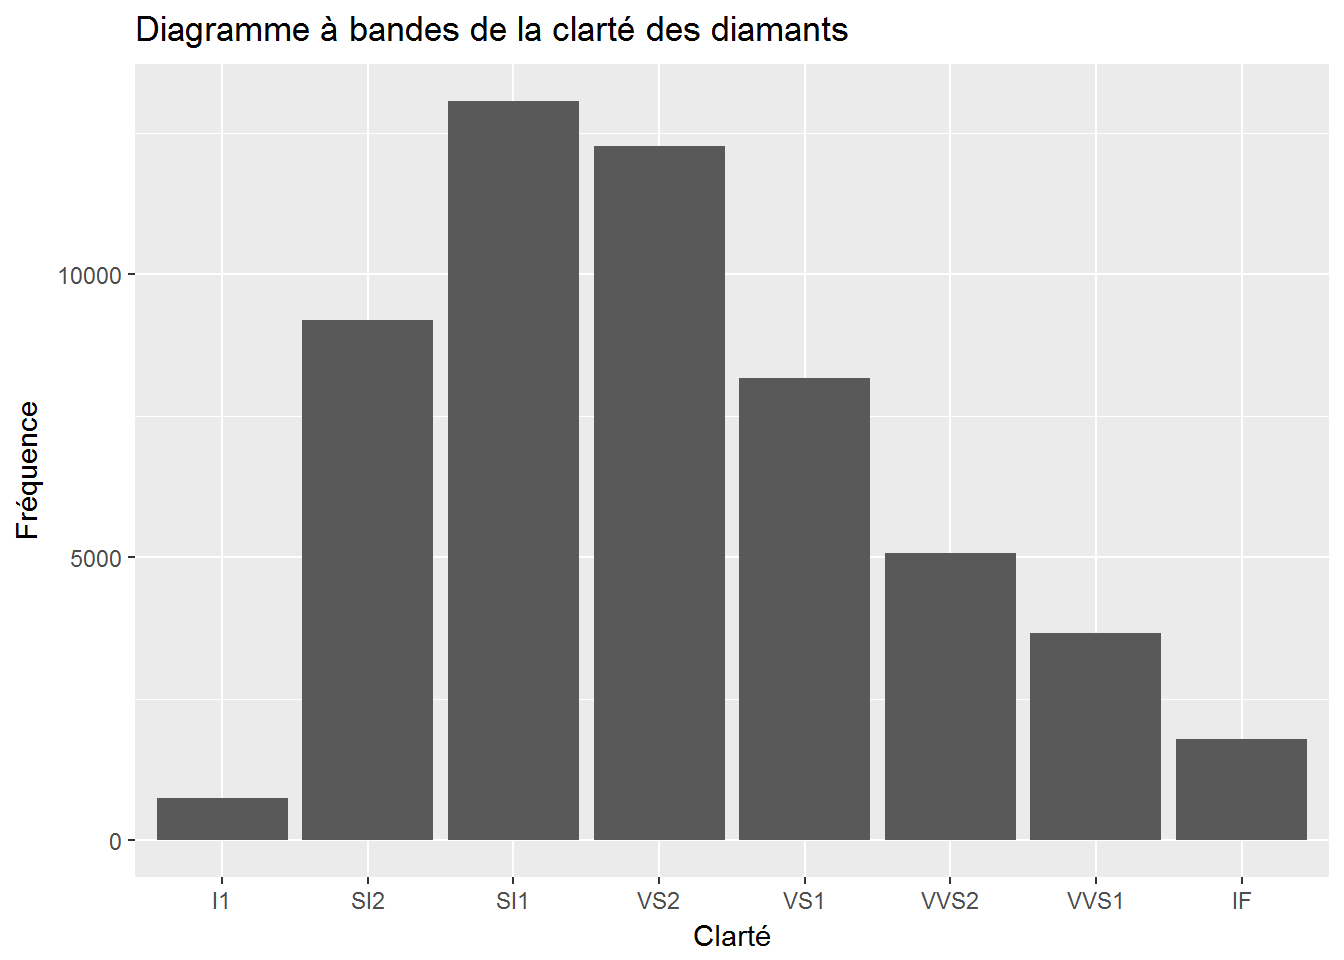
\includegraphics{02-presentation-donnees_files/figure-latex/unnamed-chunk-6-1.pdf}

Pour la variable \texttt{cut}.

\begin{Shaded}
\begin{Highlighting}[]
\KeywordTok{ggplot}\NormalTok{(diamonds, }\KeywordTok{aes}\NormalTok{(cut)) }\OperatorTok{+}\StringTok{ }\KeywordTok{geom_bar}\NormalTok{() }\OperatorTok{+}
\StringTok{  }\KeywordTok{labs}\NormalTok{(}
    \DataTypeTok{x =} \StringTok{"Coupe"}\NormalTok{, }
    \DataTypeTok{y =} \StringTok{"Fréquence"}\NormalTok{, }
    \DataTypeTok{title =} \StringTok{"Diagramme à bandes de la coupe des diamants"}\NormalTok{)}
\end{Highlighting}
\end{Shaded}

\includegraphics{02-presentation-donnees_files/figure-latex/unnamed-chunk-7-1.pdf}

\subsection{Diagramme circulaire}\label{diagramme-circulaire}

\begin{Shaded}
\begin{Highlighting}[]
\KeywordTok{ggplot}\NormalTok{(diamonds, }\KeywordTok{aes}\NormalTok{(}\DataTypeTok{x =} \KeywordTok{factor}\NormalTok{(}\DecValTok{1}\NormalTok{), }\DataTypeTok{fill =}\NormalTok{ cut)) }\OperatorTok{+}\StringTok{ }
\StringTok{  }\KeywordTok{geom_bar}\NormalTok{() }\OperatorTok{+}
\StringTok{  }\KeywordTok{coord_polar}\NormalTok{(}\DataTypeTok{theta =} \StringTok{"y"}\NormalTok{)}
\end{Highlighting}
\end{Shaded}

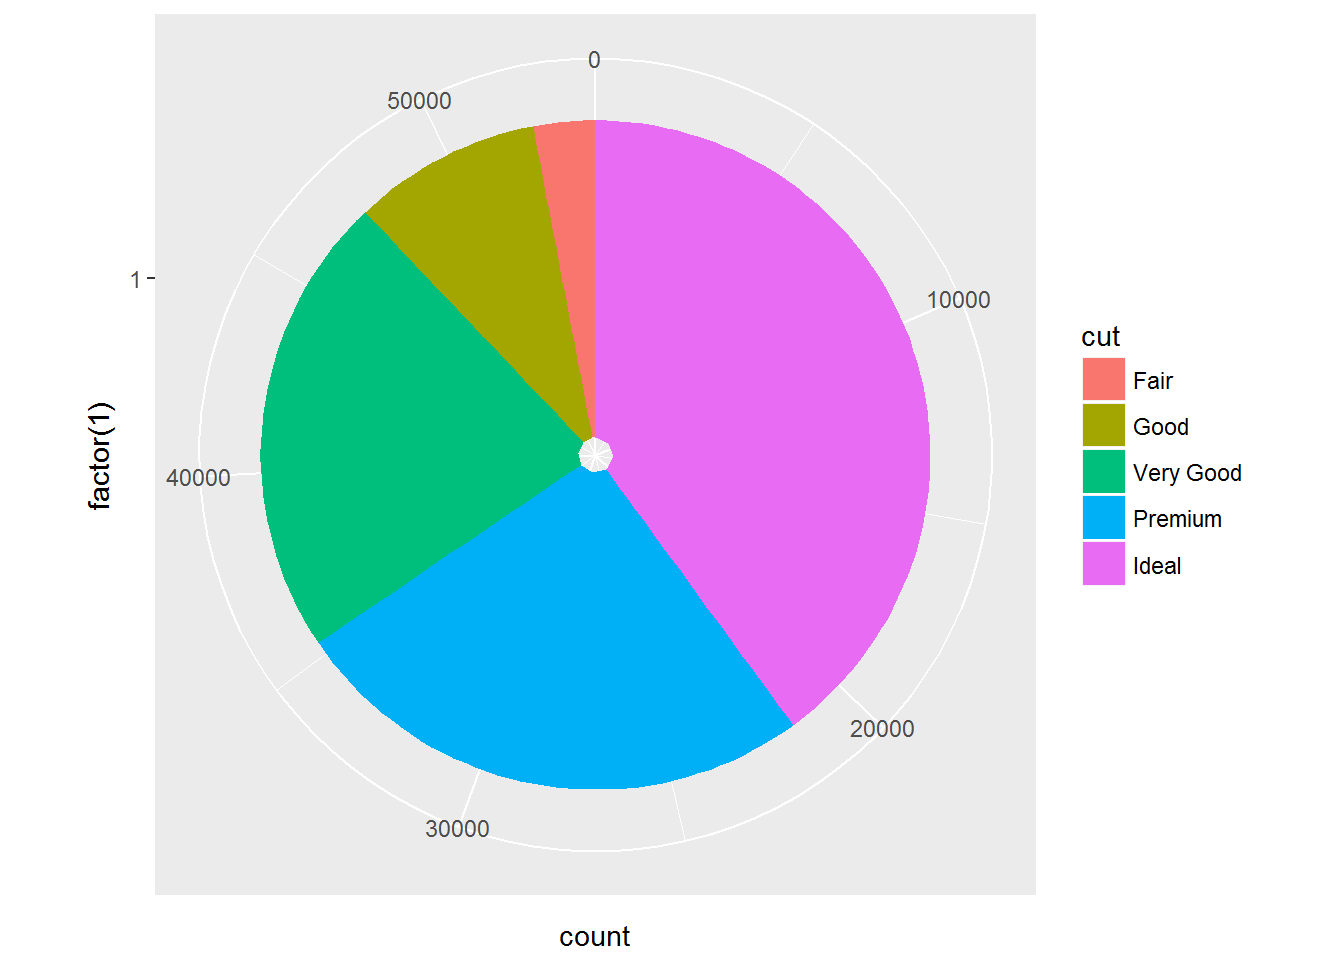
\includegraphics{02-presentation-donnees_files/figure-latex/unnamed-chunk-8-1.pdf}

\section{Variables quantitatives}\label{variables-quantitatives-1}

\subsection{Tableaux de fréquences}\label{freqquantitatives}

Pour une variable quantitative discrète, il suffit d'utiliser la
fonction \texttt{tabfreq} pour représenter les données sous forme de
tableau. Par exemple, pour la variable \texttt{cyl} de la base de
données \texttt{mtcars}.

\begin{Shaded}
\begin{Highlighting}[]
\KeywordTok{tabfreq}\NormalTok{(mtcars}\OperatorTok{$}\NormalTok{cyl)}
\end{Highlighting}
\end{Shaded}

\begin{tabular}{l|c|c|c}
\hline
mtcars\$cyl & Fréquence & Fréquence relative & Fréquence relative cumulée\\
\hline
4 & 11 & 0.344 & 0.344\\
\hline
6 & 7 & 0.219 & 0.562\\
\hline
8 & 14 & 0.438 & 1.000\\
\hline
Total & 32 & 1.000 & 1.000\\
\hline
\end{tabular}

Pour représenter une variable quantitative continue sous forme de
tableau, il faut effectuer un traitement préalable sur les données.

Étudions la variable \texttt{carat} de la base de données
\texttt{diamonds}. Si nous tentons d'utiliser la commande
\texttt{tabfreq} directement, nous allons obtenir une table beaucoup
trop grande. En effet, la variable \texttt{carat} possède 273 valeurs
différentes!

Pour représenter la variable correctement, nous allons débuter par
observer l'étendue des valeurs possibles de cette variable en utilisant
la commande \texttt{range}. Nous avons donc:

\begin{Shaded}
\begin{Highlighting}[]
\KeywordTok{range}\NormalTok{(diamonds}\OperatorTok{$}\NormalTok{carat)}
\end{Highlighting}
\end{Shaded}

\begin{verbatim}
## [1] 0.20 5.01
\end{verbatim}

La sortie de \texttt{R} signifie que la valeur la plus petite de
\texttt{carat} est 0.2, et que la plus grande est 5.01.

Nous voulons maintenant recoder notre variable \texttt{carat} pour
obtenir des classes. Dans notre exemple, il semble adéquat de créer des
classes de largeur 1 en débutant à 0 et en terminant à 6. L'option
\texttt{breaks} permet de décider des classes et l'option \texttt{right}
permet de fermer l'intervalle à gauche et de l'ouvrir à droite.

\begin{Shaded}
\begin{Highlighting}[]
\NormalTok{carat_class =}\StringTok{ }\KeywordTok{cut}\NormalTok{(diamonds}\OperatorTok{$}\NormalTok{carat,}
                  \DataTypeTok{breaks =} \KeywordTok{seq}\NormalTok{(}\DataTypeTok{from =} \DecValTok{0}\NormalTok{, }\DataTypeTok{to =} \DecValTok{6}\NormalTok{, }\DataTypeTok{by =} \DecValTok{1}\NormalTok{),}
                  \DataTypeTok{right =} \OtherTok{FALSE}\NormalTok{)}
\KeywordTok{tabfreq}\NormalTok{(carat_class)}
\end{Highlighting}
\end{Shaded}

\begin{tabular}{l|c|c|c}
\hline
carat\_class & Fréquence & Fréquence relative & Fréquence relative cumulée\\
\hline
[0,1) & 34880 & 0.647 & 0.647\\
\hline
[1,2) & 16906 & 0.313 & 0.960\\
\hline
[2,3) & 2114 & 0.039 & 0.999\\
\hline
[3,4) & 34 & 0.001 & 1.000\\
\hline
[4,5) & 5 & 0.000 & 1.000\\
\hline
[5,6) & 1 & 0.000 & 1.000\\
\hline
Total & 53940 & 1.000 & 1.000\\
\hline
\end{tabular}

\subsection{Diagramme à bâtons}\label{diagramme-a-batons}

Pour les variables quantitatives discrètes, le diagramme à bâtons est le
graphique de choix.

\begin{Shaded}
\begin{Highlighting}[]
\KeywordTok{ggplot}\NormalTok{(mtcars, }\KeywordTok{aes}\NormalTok{(cyl)) }\OperatorTok{+}\StringTok{ }
\StringTok{  }\KeywordTok{geom_bar}\NormalTok{(}\DataTypeTok{width =} \FloatTok{0.1}\NormalTok{) }\OperatorTok{+}\StringTok{ }
\StringTok{  }\KeywordTok{labs}\NormalTok{(}
    \DataTypeTok{x =} \StringTok{"Nombre de cylindres"}\NormalTok{, }
    \DataTypeTok{y =} \StringTok{"Fréquence"}\NormalTok{, }
    \DataTypeTok{title =} \StringTok{"Diagramme à bâtons du nombre de cylindres"}\NormalTok{)}
\end{Highlighting}
\end{Shaded}

\includegraphics{02-presentation-donnees_files/figure-latex/unnamed-chunk-12-1.pdf}

\subsection{Histogramme}\label{histogramme}

Pour les variables quantitatives discrètes, il est possible d'utiliser
l'histogramme.

\begin{Shaded}
\begin{Highlighting}[]
\KeywordTok{ggplot}\NormalTok{(diamonds, }\KeywordTok{aes}\NormalTok{(price)) }\OperatorTok{+}\StringTok{ }
\StringTok{  }\KeywordTok{geom_histogram}\NormalTok{(}\DataTypeTok{color =} \StringTok{"white"}\NormalTok{,}\DataTypeTok{binwidth =} \DecValTok{1000}\NormalTok{, }\DataTypeTok{center =} \DecValTok{500}\NormalTok{) }\OperatorTok{+}
\StringTok{  }\KeywordTok{labs}\NormalTok{(}
    \DataTypeTok{x =} \StringTok{"Prix"}\NormalTok{, }
    \DataTypeTok{y =} \StringTok{"Fréquence"}\NormalTok{, }
    \DataTypeTok{title =} \StringTok{"Histogramme du prix des diamants"}\NormalTok{)}
\end{Highlighting}
\end{Shaded}

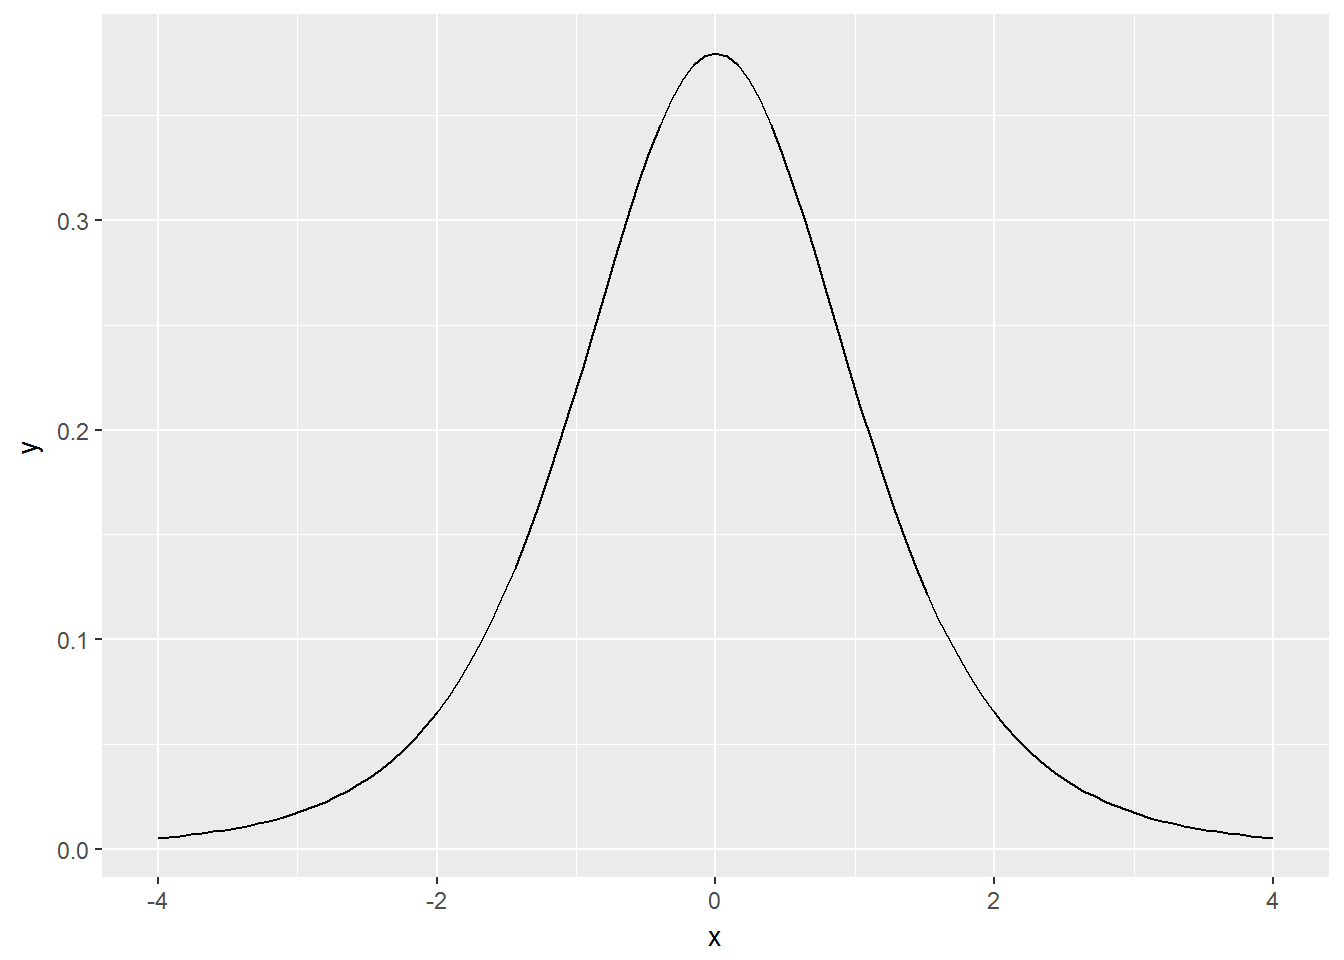
\includegraphics{02-presentation-donnees_files/figure-latex/unnamed-chunk-13-1.pdf}

\subsection{Polygone de fréquences}\label{polygone-de-frequences}

Pour les variables quantitatives discrètes, il est possible d'utiliser
le polygone de fréquences.

\begin{Shaded}
\begin{Highlighting}[]
\KeywordTok{ggplot}\NormalTok{(diamonds, }\KeywordTok{aes}\NormalTok{(price)) }\OperatorTok{+}\StringTok{ }
\StringTok{  }\KeywordTok{geom_freqpoly}\NormalTok{(}\DataTypeTok{size =} \DecValTok{1}\NormalTok{,}\DataTypeTok{binwidth =} \DecValTok{1000}\NormalTok{, }\DataTypeTok{center =} \DecValTok{500}\NormalTok{) }\OperatorTok{+}\StringTok{ }
\StringTok{  }\KeywordTok{labs}\NormalTok{(}
    \DataTypeTok{x =} \StringTok{"Prix"}\NormalTok{, }
    \DataTypeTok{y =} \StringTok{"Fréquence"}\NormalTok{, }
    \DataTypeTok{title =} \StringTok{"Polygone de fréquences du prix des diamants"}\NormalTok{)}
\end{Highlighting}
\end{Shaded}

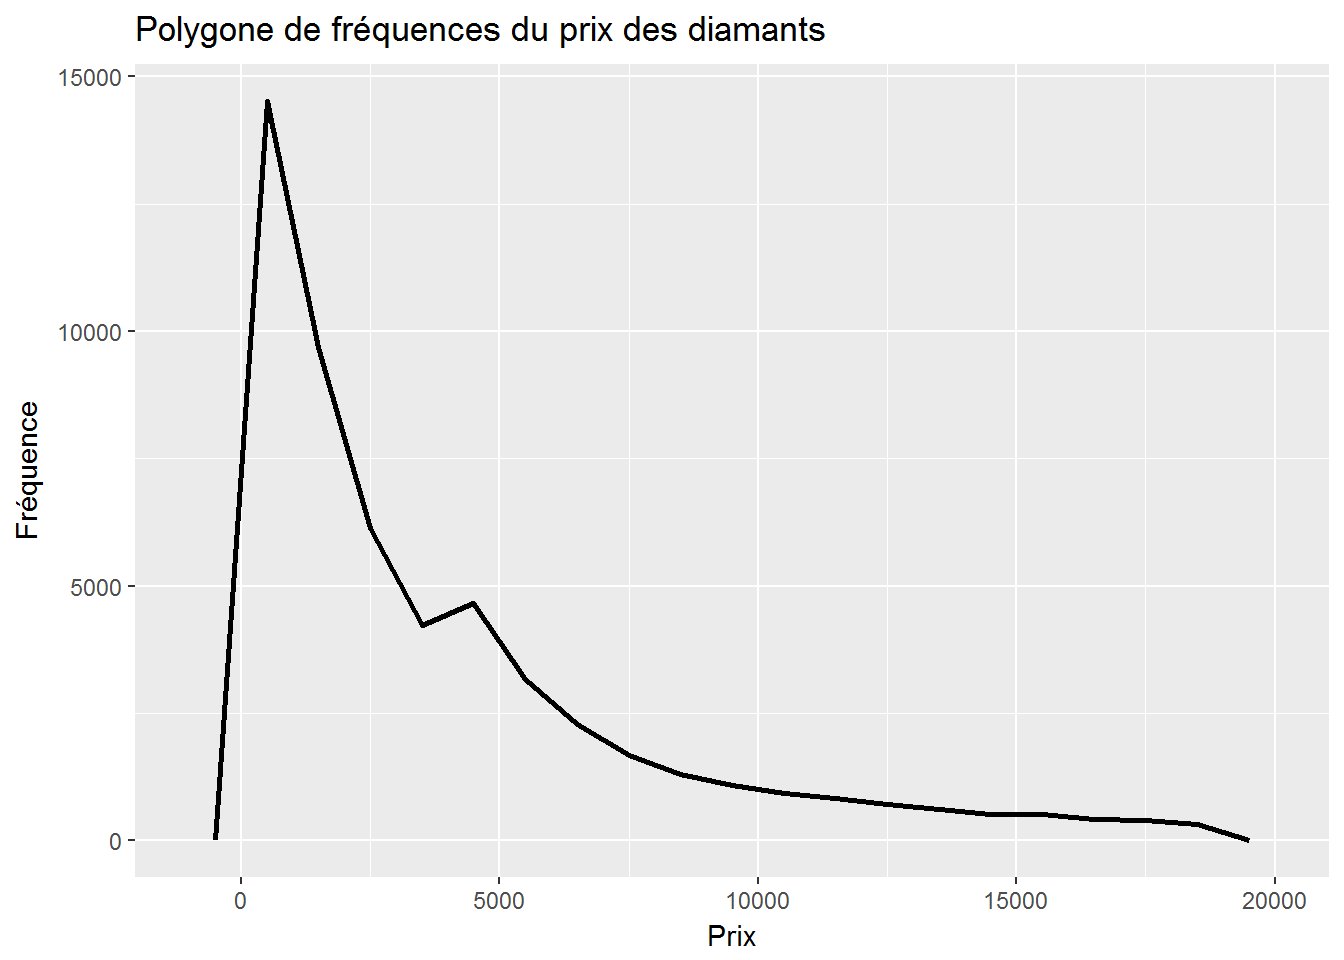
\includegraphics{02-presentation-donnees_files/figure-latex/unnamed-chunk-14-1.pdf}

\subsection{Ogive des pourcentages
cumulés}\label{ogive-des-pourcentages-cumules}

Pour les variables quantitatives discrètes, il est possible d'utiliser
l'ogive des pourcentages cumulés.

\begin{Shaded}
\begin{Highlighting}[]
\KeywordTok{ggplot}\NormalTok{(diamonds, }\KeywordTok{aes}\NormalTok{(price)) }\OperatorTok{+}\StringTok{ }
\StringTok{  }\KeywordTok{stat_ecdf}\NormalTok{(}\DataTypeTok{pad =} \OtherTok{FALSE}\NormalTok{) }\OperatorTok{+}\StringTok{ }
\StringTok{  }\KeywordTok{labs}\NormalTok{(}
    \DataTypeTok{x =} \StringTok{"Prix"}\NormalTok{, }
    \DataTypeTok{y =} \StringTok{"Fréquence relative cumulée"}\NormalTok{, }
    \DataTypeTok{title =} \StringTok{"Ogive des pourcentages cumulés du prix des diamants"}\NormalTok{)}
\end{Highlighting}
\end{Shaded}

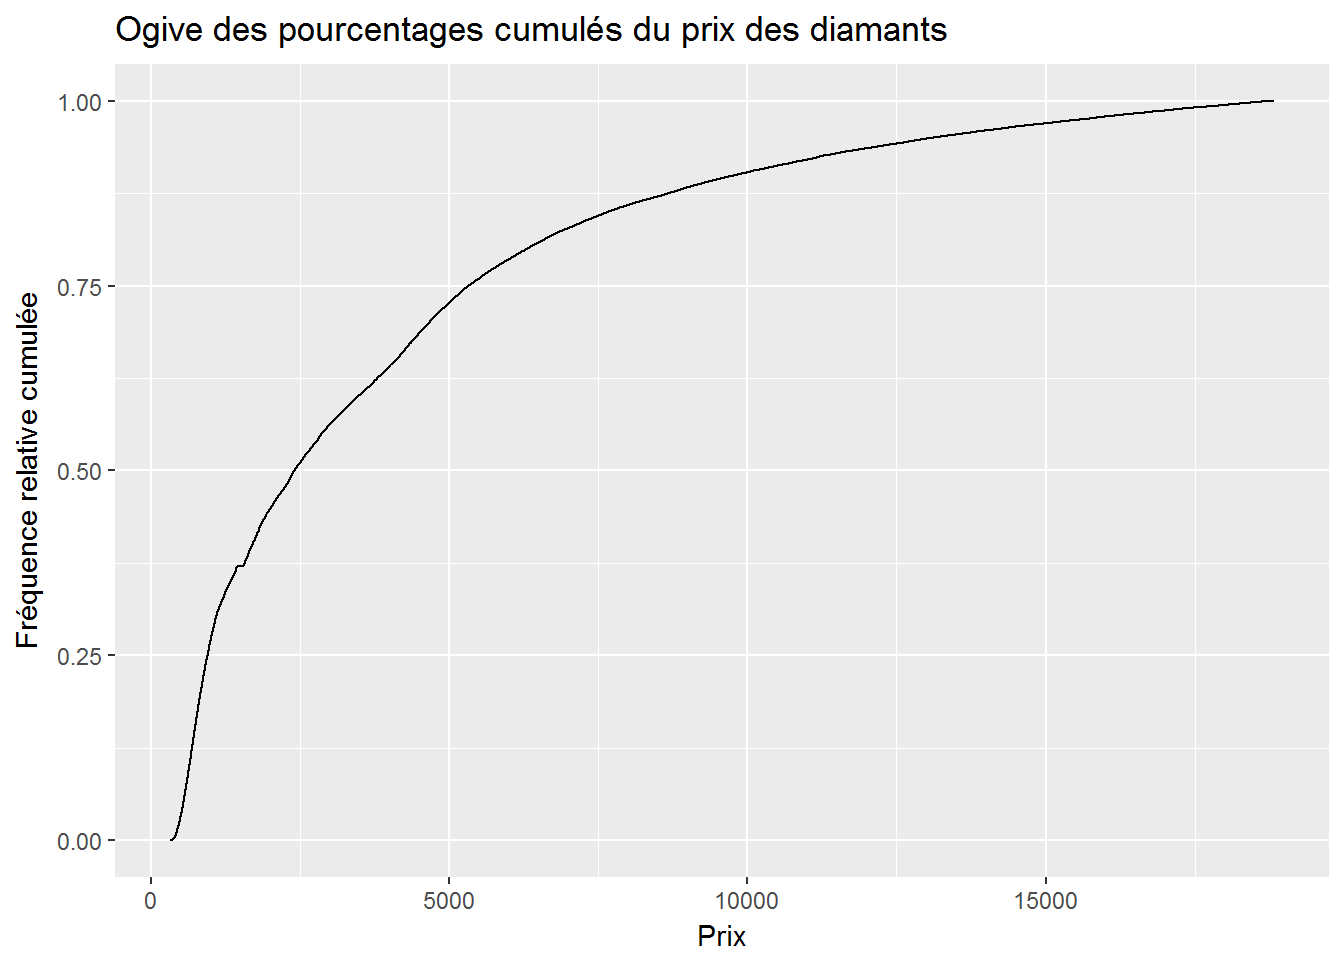
\includegraphics{02-presentation-donnees_files/figure-latex/unnamed-chunk-15-1.pdf}

\subsection{Histogramme et polygone de
fréquences}\label{histogramme-et-polygone-de-frequences}

Pour les variables quantitatives discrètes, il est possible d'utiliser
l'histogramme et le polygone de fréquences.

\begin{Shaded}
\begin{Highlighting}[]
\KeywordTok{ggplot}\NormalTok{(diamonds, }\KeywordTok{aes}\NormalTok{(price)) }\OperatorTok{+}\StringTok{ }
\StringTok{  }\KeywordTok{geom_histogram}\NormalTok{(}\DataTypeTok{color =} \StringTok{"white"}\NormalTok{,,}\DataTypeTok{binwidth =} \DecValTok{1000}\NormalTok{, }\DataTypeTok{center =} \DecValTok{500}\NormalTok{) }\OperatorTok{+}\StringTok{ }
\StringTok{  }\KeywordTok{geom_freqpoly}\NormalTok{(}\DataTypeTok{size =} \DecValTok{1}\NormalTok{,,}\DataTypeTok{binwidth =} \DecValTok{1000}\NormalTok{, }\DataTypeTok{center =} \DecValTok{500}\NormalTok{) }\OperatorTok{+}\StringTok{ }
\StringTok{  }\KeywordTok{labs}\NormalTok{(}
    \DataTypeTok{x =} \StringTok{"Prix"}\NormalTok{, }
    \DataTypeTok{y =} \StringTok{"Fréquence"}\NormalTok{, }
    \DataTypeTok{title =} \StringTok{"Histogramme et polygone de fréquences du prix des diamants"}\NormalTok{)}
\end{Highlighting}
\end{Shaded}

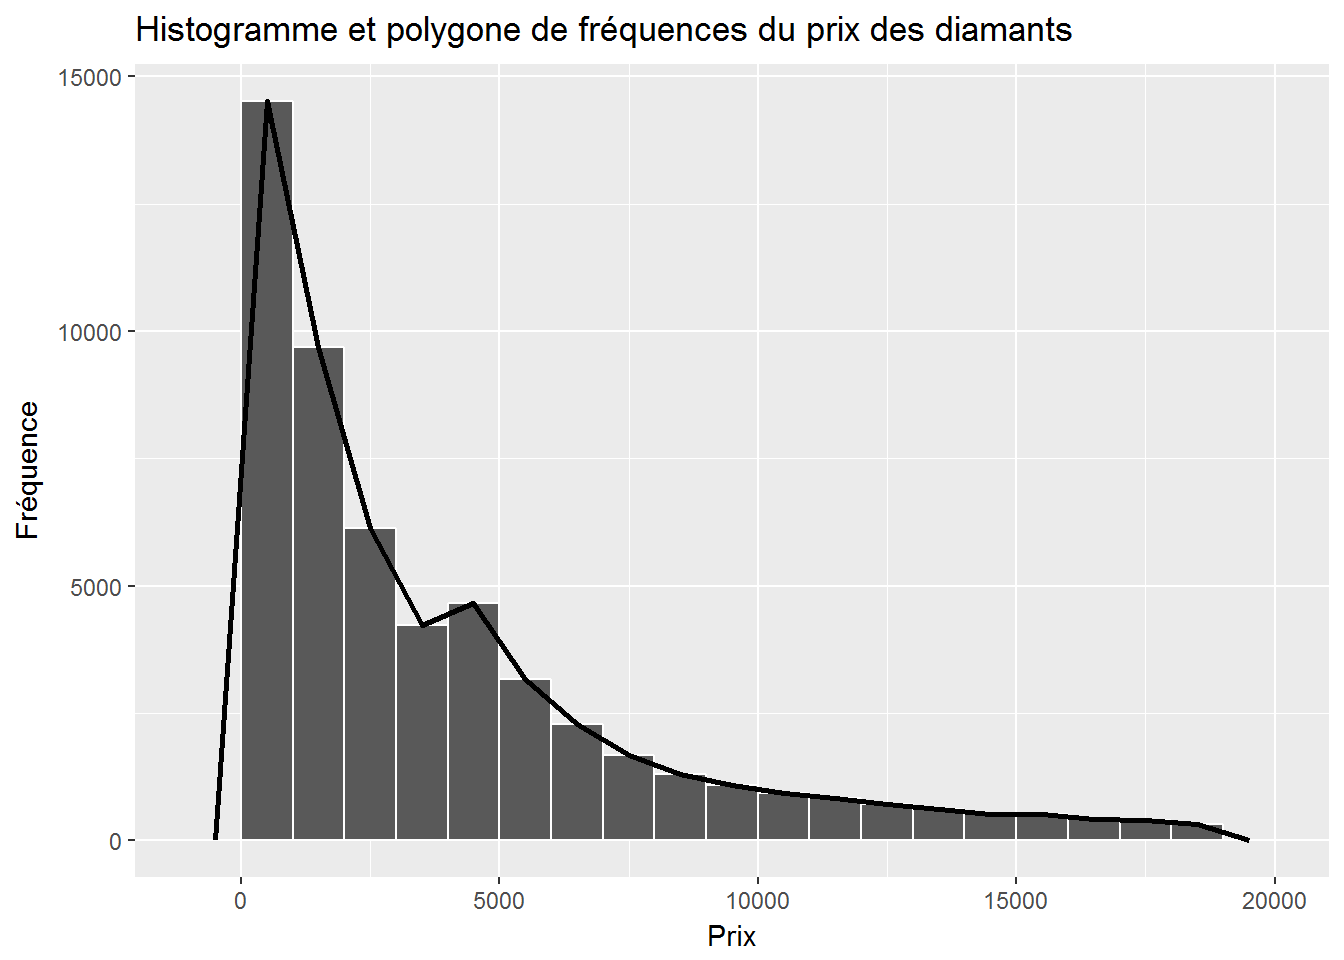
\includegraphics{02-presentation-donnees_files/figure-latex/unnamed-chunk-16-1.pdf}

\part{Les mesures associées aux
données}\label{part-les-mesures-associees-aux-donnees}

\chapter{Les différentes mesures}\label{les-differentes-mesures}

Dans ce chapitre, nous verrons comment utiliser \texttt{R} pour calculer
les mesures importantes permettant de résumer des données.

Nous allons charger les paquetages que nous allons utiliser:

\begin{Shaded}
\begin{Highlighting}[]
\KeywordTok{library}\NormalTok{(ggplot2)}
\KeywordTok{library}\NormalTok{(nycflights13)}
\end{Highlighting}
\end{Shaded}

\section{Les mesures de tendance
centrale}\label{les-mesures-de-tendance-centrale}

Les mesures de tendance centrale permettent de déterminer où se situe le
« centre » des données. Les trois mesures de tendance centrale sont le
mode, la moyenne et la médiane.

\subsection{Le mode}\label{le-mode}

Le mode est la \textbf{modalité}, \textbf{valeur} ou \textbf{classe}
possédant la plus grande fréquence. En d'autres mots, c'est la donnée la
plus fréquente.

Puisque le mode se préoccupe seulement de la donnée la plus fréquente,
il n'est pas influencé par les valeurs extrêmes.

Lorsque le mode est une classe, il est appelé \textbf{classe modale}.

Le mode est noté \textbf{Mo}.

Le langage \texttt{R} ne possède pas de fonction permettant de calculer
le mode. La façon la plus simple de le calculer est d'utiliser la
fonction \texttt{table} de \texttt{R}.

Par exemple, si nous voulons connaître le mode de la variable
\texttt{cut} de la base de données \texttt{diamonds}:

\begin{Shaded}
\begin{Highlighting}[]
\KeywordTok{table}\NormalTok{(diamonds}\OperatorTok{$}\NormalTok{cut)}
\end{Highlighting}
\end{Shaded}

\begin{verbatim}
## 
##      Fair      Good Very Good   Premium     Ideal 
##      1610      4906     12082     13791     21551
\end{verbatim}

Nous remarquons que le maximum est à la modalité \emph{Ideal} avec une
fréquence de 21551.

Si nous nous intéressons au mode d'une variable quantitative discrète
comme \texttt{cyl} de la base de données \texttt{mtcars} nous obtenons:

\begin{Shaded}
\begin{Highlighting}[]
\KeywordTok{table}\NormalTok{(mtcars}\OperatorTok{$}\NormalTok{cyl)}
\end{Highlighting}
\end{Shaded}

\begin{verbatim}
## 
##  4  6  8 
## 11  7 14
\end{verbatim}

Nous remarquons que le maximum est à la valeur \emph{8} avec une
fréquence de 14.

Dans le cas d'une variable quantitative continue, pour calculer le mode,
il faut commencer par séparer les données en classes. Nous utiliserons
les mêmes classes utilisées à la section \ref{freqquantitatives}

\begin{Shaded}
\begin{Highlighting}[]
\NormalTok{carat_class =}\StringTok{ }\KeywordTok{cut}\NormalTok{(diamonds}\OperatorTok{$}\NormalTok{carat,}
                  \DataTypeTok{breaks =} \KeywordTok{seq}\NormalTok{(}\DataTypeTok{from =} \DecValTok{0}\NormalTok{, }\DataTypeTok{to =} \DecValTok{6}\NormalTok{, }\DataTypeTok{by =} \DecValTok{1}\NormalTok{),}
                  \DataTypeTok{right =} \OtherTok{FALSE}\NormalTok{)}
\KeywordTok{table}\NormalTok{(carat_class)}
\end{Highlighting}
\end{Shaded}

\begin{verbatim}
## carat_class
## [0,1) [1,2) [2,3) [3,4) [4,5) [5,6) 
## 34880 16906  2114    34     5     1
\end{verbatim}

La classe modale est donc la classe \emph{{[}0,1)} avec une fréquence de
34880.

\subsection{La médiane}\label{la-mediane}

La médiane, notée \textbf{Md}, est la valeur qui sépare une série de
données classée en ordre croissant en deux parties égales.

La médiane étant la valeur du milieu, elle est la valeur où le
pourcentage cumulé atteint 50\%.

Puisque la médiane se préoccupe seulement de déterminer où se situe le
centre des données, elle n'est pas influencée par les valeurs extrêmes.
Elle est donc une mesure de tendance centrale plus fiable que la
moyenne.

\begin{quote}
Important : La médiane n'est définie que pour les variables
quantitatives. En effet, si vous tentez d'utiliser la médiane pour des
données autres que numériques, \texttt{R} vous donnera un message
d'erreur.
\end{quote}

La fonction \texttt{median} permet de calculer la médiane en langage
\texttt{R}.

Par exemple, pour calculer la médiane de la variable \texttt{carat} de
la base de données \texttt{diamonds}, nous avons:

\begin{Shaded}
\begin{Highlighting}[]
\KeywordTok{median}\NormalTok{(diamonds}\OperatorTok{$}\NormalTok{carat)}
\end{Highlighting}
\end{Shaded}

\begin{verbatim}
## [1] 0.7
\end{verbatim}

Ceci signifie que 50\% des diamants ont une valeur en carat inférieure
ou égale à 0.7 et que 50\% des diamants ont une valeur en carat
supérieure ou égale à 0.7.

Nous pouvons aussi obtenir que la médiane de la variable \texttt{price}
de la base de données \texttt{diamonds} est donnée par:

\begin{Shaded}
\begin{Highlighting}[]
\KeywordTok{median}\NormalTok{(diamonds}\OperatorTok{$}\NormalTok{price)}
\end{Highlighting}
\end{Shaded}

\begin{verbatim}
## [1] 2401
\end{verbatim}

\subsection{La moyenne}\label{la-moyenne}

La moyenne est la valeur qui pourrait remplacer chacune des données
d'une série pour que leur somme demeure identique. Intuitivement, elle
représente le centre d'équilibre d'une série de données. La somme des
distances qui sépare les données plus petites que la moyenne devrait
être la même que la somme des distances qui sépare les données plus
grandes.

\begin{quote}
Important : La moyenne n'est définie que pour les variables
quantitatives. En effet, si vous tentez d'utiliser la moyenne pour des
données autres que numériques, \texttt{R} vous donnera un message
d'erreur.
\end{quote}

La fonction \texttt{mean} permet de calculer la moyenne en langage
\texttt{R}.

Par exemple, pour calculer la moyenne de la variable \texttt{carat} de
la base de données \texttt{diamonds}, nous avons:

\begin{Shaded}
\begin{Highlighting}[]
\KeywordTok{mean}\NormalTok{(diamonds}\OperatorTok{$}\NormalTok{carat)}
\end{Highlighting}
\end{Shaded}

\begin{verbatim}
## [1] 0.7979397
\end{verbatim}

Nous pouvons aussi obtenir que la moyenne de la variable \texttt{price}
de la base de données \texttt{diamonds} est donnée par:

\begin{Shaded}
\begin{Highlighting}[]
\KeywordTok{mean}\NormalTok{(diamonds}\OperatorTok{$}\NormalTok{price)}
\end{Highlighting}
\end{Shaded}

\begin{verbatim}
## [1] 3932.8
\end{verbatim}

\section{Les mesures de dispersion}\label{les-mesures-de-dispersion}

Les mesures de tendance centrale (mode, moyenne et médiane) ne
permettent pas de déterminer si une série de données est principalement
située autour de son centre, ou si au contraire elle est très dispersée.

Les mesures de dispersion, elles, permettent de déterminer si une série
de données est centralisée autour de sa moyenne, ou si elle est au
contraire très dispersée.

Les mesures de dispersion sont l'étendue, la variance, l'écart-type et
le coefficient de variation.

\subsection{L'étendue}\label{letendue}

La première mesure de dispersion, l'étendue, est la différence entre la
valeur maximale et la valeur minimale.

L'étendue ne tenant compte que du maximum et du minimum, elle est
grandement influencée par les valeurs extrêmes. Elle est donc une mesure
de dispersion peu fiable.

La fonction \texttt{range} permet de calculer l'étendue d'une variable
en langage \texttt{R}.

Par exemple, pour calculer l'étendue de la variable \texttt{carat} de la
base de données \texttt{diamonds}, nous avons:

\begin{Shaded}
\begin{Highlighting}[]
\KeywordTok{range}\NormalTok{(diamonds}\OperatorTok{$}\NormalTok{carat)}
\end{Highlighting}
\end{Shaded}

\begin{verbatim}
## [1] 0.20 5.01
\end{verbatim}

Nous pouvons donc calculer l'étendue de la variable \texttt{carat} en
soustrayant les deux valeurs obtenues par la fonction \texttt{range},
c'est-à-dire que l'étendue est 5.01-0.2 = 4.81.

\subsection{La variance}\label{la-variance}

La variance sert principalement à calculer l'écart-type, la mesure de
dispersion la plus connue.

\begin{quote}
Attention : Les unités de la variance sont des
unités\textsuperscript{2}.
\end{quote}

La fonction \texttt{var} permet de calculer la variance d'une variable
en langage \texttt{R}.

Par exemple, pour calculer la variance de la variable \texttt{carat} de
la base de données \texttt{diamonds}, nous avons:

\begin{Shaded}
\begin{Highlighting}[]
\KeywordTok{var}\NormalTok{(diamonds}\OperatorTok{$}\NormalTok{carat)}
\end{Highlighting}
\end{Shaded}

\begin{verbatim}
## [1] 0.2246867
\end{verbatim}

Ceci signifie que la variance de la variable \texttt{carat} est
0.2246867 carat\textsuperscript{2}.

\subsection{L'écart-type}\label{lecart-type}

L'écart-type est la mesure de dispersion la plus couramment utilisée. Il
peut être vu comme la « moyenne » des écarts entre les données et la
moyenne.

Puisque l'écart-type tient compte de chacune des données, il est une
mesure de dispersion beaucoup plus fiable que l'étendue.

Il est défini comme la racine carrée de la variance.

La fonction \texttt{sd} permet de calculer l''écart-type d'une variable
en langage \texttt{R}.

Par exemple, pour calculer l'écart-type de la variable \texttt{carat} de
la base de données \texttt{diamonds}, nous avons:

\begin{Shaded}
\begin{Highlighting}[]
\KeywordTok{sd}\NormalTok{(diamonds}\OperatorTok{$}\NormalTok{carat)}
\end{Highlighting}
\end{Shaded}

\begin{verbatim}
## [1] 0.4740112
\end{verbatim}

Ceci signifie que l'écart-type de la variable \texttt{carat} est
0.4740112 carat.

\subsection{Le coefficient de
variation}\label{le-coefficient-de-variation}

Le coefficient de variation, noté C. V., est calculé comme suit :

\begin{equation}
C.V. = \dfrac{\text{ecart-type}}{\text{moyenne}}\times 100\%
\end{equation}

Si le coefficient est inférieur à 15\%, les données sont dites
\textbf{homogènes}. Cela veut dire que les données sont situées près les
unes des autres.

Dans le cas contraire, les données sont dites \textbf{hétérogènes}. Cela
veut dire que les données sont très dispersées.

\begin{quote}
Important : Le coefficient de variation ne possède pas d'unité, outre le
symbole de pourcentage.
\end{quote}

Il n'existe pas de fonctions en \texttt{R} permettant de calculer
directement le coefficient de variation. Par contre, nous pouvons
utiliser en conjonction les fonctions \texttt{sd} et \texttt{mean} pour
le calculer.

Par exemple, pour calculer le coefficient de variation de la variable
\texttt{carat} de la base de données \texttt{diamonds}, nous avons:

\begin{Shaded}
\begin{Highlighting}[]
\KeywordTok{sd}\NormalTok{(diamonds}\OperatorTok{$}\NormalTok{carat)}\OperatorTok{/}\KeywordTok{mean}\NormalTok{(diamonds}\OperatorTok{$}\NormalTok{carat)}\OperatorTok{*}\DecValTok{100}
\end{Highlighting}
\end{Shaded}

\begin{verbatim}
## [1] 59.40439
\end{verbatim}

Le C.V. de la variable \texttt{carat} est donc 59.4043906 \%, ce qui
signifie que les données sont hétérogènes, car le coefficient de
variation est plus grand que 15\%.

\section{Les mesures de position}\label{les-mesures-de-position}

Les mesures de position permettent de situer une donnée par rapport aux
autres. Les différentes mesures de position sont la cote Z, les
quantiles et les rangs.

Tout comme les mesures de dispersion, celles-ci ne sont définies que
pour une variable quantitative.

\subsection{La cote z}\label{la-cote-z}

Cette mesure de position se base sur la moyenne et l'écart-type.

La cote Z d'une donnée x est calculée comme suit :

\begin{equation}
Z = \dfrac{x-\text{moyenne}}{\text{ecart-type}}
\end{equation}

\begin{quote}
Important : La cote z ne possède pas d'unités.
\end{quote}

Une cote Z peut être positive, négative ou nulle.

\begin{longtable}[]{@{}rl@{}}
\toprule
Cote Z & Interprétation\tabularnewline
\midrule
\endhead
Z\textgreater{}0 & donnée supérieure à la moyenne\tabularnewline
Z\textless{}0 & donnée inférieure à la moyenne\tabularnewline
Z=0 & donnée égale à la moyenne\tabularnewline
\bottomrule
\end{longtable}

Il n'existe pas de fonctions en \texttt{R} permettant de calculer
directement la cote Z. Par contre, nous pouvons utiliser en conjonction
les fonctions \texttt{sd} et \texttt{mean} pour la calculer.

Par exemple, si nous voulons calculer la cote Z d'un diamant de 3
carats, nous avons:

\begin{Shaded}
\begin{Highlighting}[]
\NormalTok{(}\DecValTok{3}\OperatorTok{-}\KeywordTok{mean}\NormalTok{(diamonds}\OperatorTok{$}\NormalTok{carat))}\OperatorTok{/}\KeywordTok{sd}\NormalTok{(diamonds}\OperatorTok{$}\NormalTok{carat)}
\end{Highlighting}
\end{Shaded}

\begin{verbatim}
## [1] 4.645587
\end{verbatim}

\subsection{Les quantiles}\label{les-quantiles}

Un quantile est une donnée qui correspond à un certain pourcentage
cumulé.

Parmi les quantiles, on distingue les quartiles, les quintiles, les
déciles et les centiles.

\begin{itemize}
\tightlist
\item
  Les quartiles Q\textsubscript{1}, Q\textsubscript{2} et
  Q\textsubscript{3}, séparent les données en quatre parties égales.
  Environ 25\% des données sont inférieures ou égales à
  Q\textsubscript{1}. Environ 50\% des données sont inférieures ou
  égales à Q\textsubscript{2}. Environ 75\% des données sont inférieures
  ou égales à Q\textsubscript{3}.
\item
  Les quintiles V\textsubscript{1}, V\textsubscript{2},
  V\textsubscript{3} et V\textsubscript{4}, séparent les données en cinq
  parties égales. Environ 20\% des données sont inférieures ou égales à
  V\textsubscript{1}. Environ 40\% des données sont inférieures ou
  égales à V\textsubscript{2}. Etc.
\item
  Les déciles D\textsubscript{1}, D\textsubscript{2}, \ldots{},
  D\textsubscript{8} et D\textsubscript{9}, séparent les données en dix
  parties égales. Environ 10\% des données sont inférieures ou égales à
  D\textsubscript{1}. Environ 20\% des données sont inférieures ou
  égales à D\textsubscript{2}. Etc.
\item
  Les centiles C\textsubscript{1}, C\textsubscript{2}, \ldots{},
  C\textsubscript{98} et C\textsubscript{99}, séparent les données en
  cent parties égales. Environ 1\% des données sont inférieures ou
  égales à C\textsubscript{1}. Environ 2\% des données sont inférieures
  ou égales à C\textsubscript{2}. Etc.
\end{itemize}

\begin{quote}
Il est utile de noter que certains quantiles se recoupent.
\end{quote}

La fonction \texttt{quantile} permet de calculer n'importe quel quantile
d'une variable en langage \texttt{R}. Il suffit d'indiquer la variable
étudiée ainsi que le pourcentage du quantile voulu.

Par exemple, si nous voulons calculer D\textsubscript{1} pour la
variable \texttt{carat}, nous allons utiliser la fonction
\texttt{quantile} avec une probabilité de 0,1.

\begin{Shaded}
\begin{Highlighting}[]
\KeywordTok{quantile}\NormalTok{(diamonds}\OperatorTok{$}\NormalTok{carat, }\FloatTok{0.1}\NormalTok{)}
\end{Highlighting}
\end{Shaded}

\begin{verbatim}
##  10% 
## 0.31
\end{verbatim}

Ceci implique que 10\% des diamants ont une valeur en carat inférieure
ou égale à 0.31 carat.

Nous pouvons calculer le troisième quartile Q\textsubscript{3} de la
variable \texttt{price} en utilisant la fonction \texttt{quantile} avec
une probabilité de 0,75.

\begin{Shaded}
\begin{Highlighting}[]
\KeywordTok{quantile}\NormalTok{(diamonds}\OperatorTok{$}\NormalTok{price, }\FloatTok{0.75}\NormalTok{)}
\end{Highlighting}
\end{Shaded}

\begin{verbatim}
##     75% 
## 5324.25
\end{verbatim}

Ceci implique que 75\% des diamants ont un prix en dollars inférieur ou
égal à 5324.25 \$.

\subsection{\texorpdfstring{La commande
\texttt{summary}}{La commande summary}}\label{la-commande-summary}

La commande \texttt{summary} produit un sommaire contenant six mesures
importantes:

\begin{enumerate}
\def\labelenumi{\arabic{enumi}.}
\tightlist
\item
  \texttt{Min} : le minimum de la variable
\item
  \texttt{1st\ Qu.}: Le premier quartile, Q\textsubscript{1}, de la
  variable
\item
  \texttt{Median} : La médiane de la variable
\item
  \texttt{Mean} : La moyenne de la variable
\item
  \texttt{3rd\ Qu.} : Le troisième quartile, Q\textsubscript{3}, de la
  variable
\item
  \texttt{Max} : Le maximum de la variable
\end{enumerate}

Nous pouvons donc produire le sommaire de la variable \texttt{price} de
la base de données \texttt{diamonds} de la façon suivante:

\begin{Shaded}
\begin{Highlighting}[]
\KeywordTok{summary}\NormalTok{(diamonds}\OperatorTok{$}\NormalTok{price)}
\end{Highlighting}
\end{Shaded}

\begin{verbatim}
##    Min. 1st Qu.  Median    Mean 3rd Qu.    Max. 
##     326     950    2401    3933    5324   18823
\end{verbatim}

\subsection{Le rang centile}\label{le-rang-centile}

Un rang centile représente le pourcentage cumulé, \emph{exprimé en
nombre entier}, qui correspond à une certaine donnée. Nous déterminerons
les rangs centiles pour les variables continues seulement.

Les rangs centiles sont donc exactement l'inverse des centiles.

Il n'existe pas de fonctions dans \texttt{R} permettant de trouver
directement le rang centile, mais il est facile d'utiliser la fonction
\texttt{mean} pour le trouver.

Par exemple, si nous voulons trouver le rang centile d'un diamant qui
coûte 500\$, il suffit d'utiliser la commande suivante. La commande
calcule la moyenne de toutes les valeurs en dollars des diamants coûtant
500\$ ou moins.

\begin{Shaded}
\begin{Highlighting}[]
\KeywordTok{mean}\NormalTok{(diamonds}\OperatorTok{$}\NormalTok{price}\OperatorTok{<=}\DecValTok{500}\NormalTok{)}
\end{Highlighting}
\end{Shaded}

\begin{verbatim}
## [1] 0.03242492
\end{verbatim}

Ceci signifie que pour un diamant de 500\$, il y a 3.2424917 \% des
diamants qui ont une valeur égale ou inférieure.

\chapter{Les séries chronologiques}\label{les-series-chronologiques}

Débutons par charger les paquetages qui nous seront utiles.

\begin{Shaded}
\begin{Highlighting}[]
\KeywordTok{library}\NormalTok{(gapminder)}
\KeywordTok{library}\NormalTok{(nycflights13)}
\KeywordTok{library}\NormalTok{(ggplot2)}
\KeywordTok{library}\NormalTok{(dplyr)}
\end{Highlighting}
\end{Shaded}

\begin{verbatim}
## 
## Attachement du package : 'dplyr'
\end{verbatim}

\begin{verbatim}
## The following objects are masked from 'package:stats':
## 
##     filter, lag
\end{verbatim}

\begin{verbatim}
## The following objects are masked from 'package:base':
## 
##     intersect, setdiff, setequal, union
\end{verbatim}

Une série chronologique est un ensemble de valeurs observées d'une
variable quantitative. Elle permet d'analyser l'évolution de cette
variable dans le temps dans le but éventuel de faire des prévisions.

\section{Les graphiques}\label{les-graphiques}

Nous allons débuter par utiliser la base de données
\texttt{nycflights13}. Nous allons étudier la température au mois de
janvier 2013 à l'aéroport Newark (code ``EWR'' dans la variable
\texttt{origin}). La variable \texttt{weather} de la base de données
contient ces informations mais nous devons tout d'abord filtrer les
données pour ne conserver que celles qui correspondent à Newark et au
mois de janvier.

La commande suivante permet de faire ce filtrage. Vous n'avez pas besoin
de comprendre la syntaxe.

\begin{Shaded}
\begin{Highlighting}[]
\NormalTok{meteo_janvier_ewr <-}\StringTok{ }\NormalTok{weather }\OperatorTok\StringTok{ }
\StringTok{  }\KeywordTok{filter}\NormalTok{(origin }\OperatorTok{==}\StringTok{ "EWR"} \OperatorTok{&}\StringTok{ }\NormalTok{month }\OperatorTok{==}\StringTok{ }\DecValTok{1}\NormalTok{ )}
\end{Highlighting}
\end{Shaded}

Nous pouvons maintenant tracer les données obtenues:

\begin{Shaded}
\begin{Highlighting}[]
\KeywordTok{ggplot}\NormalTok{(meteo_janvier_ewr, }\KeywordTok{aes}\NormalTok{(}\DataTypeTok{x =}\NormalTok{ time_hour, }\DataTypeTok{y =}\NormalTok{ temp)) }\OperatorTok{+}
\StringTok{  }\KeywordTok{geom_line}\NormalTok{() }\OperatorTok{+}
\StringTok{  }\KeywordTok{geom_point}\NormalTok{() }\OperatorTok{+}
\StringTok{  }\KeywordTok{labs}\NormalTok{(}
    \DataTypeTok{x =} \StringTok{"Heures du mois de janvier"}\NormalTok{,}
    \DataTypeTok{y =} \StringTok{"Température en degrée Farhenheit"}\NormalTok{,}
    \DataTypeTok{title =} \StringTok{"Répartition de la température au mois de janvier en fonction de l'heure"}
\NormalTok{  )}
\end{Highlighting}
\end{Shaded}

\includegraphics{04-series-chronologiques_files/figure-latex/unnamed-chunk-3-1.pdf}

Nous pouvons aussi utiliser la paquetage \texttt{gapminder} qui contient
des données sur l'espérance de vie. Comme précédemment, nous allons
débuter par filtrer les données provenant uniquement du Canada.

\begin{Shaded}
\begin{Highlighting}[]
\NormalTok{gap_canada <-}\StringTok{ }\NormalTok{gapminder }\OperatorTok
\StringTok{  }\KeywordTok{filter}\NormalTok{(country }\OperatorTok{==}\StringTok{ "Canada"}\NormalTok{)}
\end{Highlighting}
\end{Shaded}

Nous pouvons maintenant tracer les données obtenues:

\begin{Shaded}
\begin{Highlighting}[]
\KeywordTok{ggplot}\NormalTok{(gap_canada, }\KeywordTok{aes}\NormalTok{(}\DataTypeTok{x =}\NormalTok{ year, }\DataTypeTok{y =}\NormalTok{ lifeExp)) }\OperatorTok{+}\StringTok{ }
\StringTok{  }\KeywordTok{geom_line}\NormalTok{() }\OperatorTok{+}\StringTok{ }\KeywordTok{geom_point}\NormalTok{() }\OperatorTok{+}
\StringTok{  }\KeywordTok{labs}\NormalTok{(}
    \DataTypeTok{x =} \StringTok{"Année"}\NormalTok{,}
    \DataTypeTok{y =} \StringTok{"Espérance de vie"}\NormalTok{,}
    \DataTypeTok{title =} \StringTok{"Répartition de l'espérance de vie au Canada en fonction de l'année"}\NormalTok{)}
\end{Highlighting}
\end{Shaded}

\includegraphics{04-series-chronologiques_files/figure-latex/unnamed-chunk-5-1.pdf}

\section{Les mesures}\label{les-mesures}

\subsection{La variation absolue}\label{la-variation-absolue}

La variation absolue mesure l'augmentation (ou la diminution) subie par
une variable dans le temps. Pour calculer la variation absolue entre un
moment A antérieur à un moment B, on utilise la formule ci-dessous :

\begin{equation}
\Delta V = V_B - V_A
\end{equation}

où V\textsubscript{B} est la valeur de la variable au temps B et
V\textsubscript{A} est la valeur de la variable au temps A.

\begin{quote}
Remarque : Les unités de la variation absolue sont les mêmes que celles
de la variable étudiée.
\end{quote}

Si nous voulons connaître la variation absolue de la population du
Canada, nous allons devoir ajouter une colonne à notre base de données
\texttt{gap\_canada}. Encore une fois, il n'est pas nécessaire de
comprendre la syntaxe. Nous ajoutons une colonne variation absolue,
notée \texttt{var\_abs}, à notre base de données \texttt{gap\_canada}.

\begin{Shaded}
\begin{Highlighting}[]
\NormalTok{gap_canada <-}\StringTok{ }\NormalTok{gap_canada }\OperatorTok
\StringTok{  }\KeywordTok{mutate}\NormalTok{(}\DataTypeTok{var_abs =}\NormalTok{ pop }\OperatorTok{-}\StringTok{ }\KeywordTok{lag}\NormalTok{(pop))}
\end{Highlighting}
\end{Shaded}

Nous pouvons maintenant représenter la variable à l'aide d'un graphique.

\begin{Shaded}
\begin{Highlighting}[]
\KeywordTok{ggplot}\NormalTok{(gap_canada, }\KeywordTok{aes}\NormalTok{(}\DataTypeTok{x =}\NormalTok{ year, }\DataTypeTok{y =}\NormalTok{ var_abs)) }\OperatorTok{+}
\StringTok{  }\KeywordTok{geom_line}\NormalTok{() }\OperatorTok{+}
\StringTok{  }\KeywordTok{geom_point}\NormalTok{() }\OperatorTok{+}
\StringTok{  }\KeywordTok{labs}\NormalTok{(}
    \DataTypeTok{x =} \StringTok{"Année"}\NormalTok{,}
    \DataTypeTok{y =} \StringTok{"Variation absolue de la population"}\NormalTok{,}
    \DataTypeTok{title =} \StringTok{"Répartition de la variation absolue de la population du Canada selon l'année"}
\NormalTok{  )}
\end{Highlighting}
\end{Shaded}

\includegraphics{04-series-chronologiques_files/figure-latex/unnamed-chunk-7-1.pdf}

\subsection{La variation moyenne}\label{la-variation-moyenne}

La variation moyenne mesure l'augmentation (ou la diminution) moyenne
subie par une variable par unité de temps. La variation moyenne entre
les moments 𝐴 et 𝐵 est donnée par :

\begin{equation}
\Delta V_{moy} = \dfrac{V_B - V_A}{B-A}
\end{equation}

\begin{quote}
Remarque : Les unités de la variation moyenne sont les unités de la
variable étudiée par unité de temps.
\end{quote}

Si nous voulons connaître la variation moyenne de la population du
Canada, nous allons devoir ajouter une colonne à notre base de données
\texttt{gap\_canada}. Encore une fois, il n'est pas nécessaire de
comprendre la syntaxe. Nous ajoutons une colonne variation moyenne,
notée \texttt{var\_moy}, à notre base de données \texttt{gap\_canada}.

\begin{Shaded}
\begin{Highlighting}[]
\NormalTok{gap_canada <-}\StringTok{ }\NormalTok{gap_canada }\OperatorTok
\StringTok{  }\KeywordTok{mutate}\NormalTok{(}\DataTypeTok{var_moy =}\NormalTok{ (pop }\OperatorTok{-}\StringTok{ }\KeywordTok{lag}\NormalTok{(pop))}\OperatorTok{/}\NormalTok{(year}\OperatorTok{-}\KeywordTok{lag}\NormalTok{(year)))}
\end{Highlighting}
\end{Shaded}

Nous pouvons maintenant représenter la variable à l'aide d'un graphique.

\begin{Shaded}
\begin{Highlighting}[]
\KeywordTok{ggplot}\NormalTok{(gap_canada, }\KeywordTok{aes}\NormalTok{(}\DataTypeTok{x =}\NormalTok{ year, }\DataTypeTok{y =}\NormalTok{ var_moy)) }\OperatorTok{+}
\StringTok{  }\KeywordTok{geom_line}\NormalTok{() }\OperatorTok{+}
\StringTok{  }\KeywordTok{geom_point}\NormalTok{() }\OperatorTok{+}
\StringTok{  }\KeywordTok{labs}\NormalTok{(}
    \DataTypeTok{x =} \StringTok{"Année"}\NormalTok{,}
    \DataTypeTok{y =} \StringTok{"Variation moyenne de la population"}\NormalTok{,}
    \DataTypeTok{title =} \StringTok{"Répartition de la variation moyenne de la population du Canada selon l'année"}
\NormalTok{  )}
\end{Highlighting}
\end{Shaded}

\includegraphics{04-series-chronologiques_files/figure-latex/unnamed-chunk-9-1.pdf}

\subsection{La variation relative (pourcentage de
variation)}\label{la-variation-relative-pourcentage-de-variation}

La variation relative exprime \emph{en pourcentage} la variation subie
par une variable entre les moments 𝐴 et 𝐵. Le pourcentageest donné par:

\begin{equation}
\Delta V_{\%} = \dfrac{V_B - V_A}{V_A}\times 100
\end{equation}

\begin{quote}
Remarque : Il n'y a pas d'unité autre que le symbole de pourcentage.
\end{quote}

Si nous voulons connaître la variation relative de la population du
Canada, nous allons devoir ajouter une colonne à notre base de données
\texttt{gap\_canada}. Encore une fois, il n'est pas nécessaire de
comprendre la syntaxe. Nous ajoutons une colonne variation relative,
notée \texttt{var\_rel}, à notre base de données \texttt{gap\_canada}.

\begin{Shaded}
\begin{Highlighting}[]
\NormalTok{gap_canada <-}\StringTok{ }\NormalTok{gap_canada }\OperatorTok
\StringTok{  }\KeywordTok{mutate}\NormalTok{(}\DataTypeTok{var_rel =}\NormalTok{ (pop }\OperatorTok{-}\StringTok{ }\KeywordTok{lag}\NormalTok{(pop))}\OperatorTok{/}\KeywordTok{lag}\NormalTok{(pop) }\OperatorTok{*}\StringTok{ }\DecValTok{100}\NormalTok{)}
\end{Highlighting}
\end{Shaded}

Nous pouvons maintenant représenter la variable à l'aide d'un graphique.

\begin{Shaded}
\begin{Highlighting}[]
\KeywordTok{ggplot}\NormalTok{(gap_canada, }\KeywordTok{aes}\NormalTok{(}\DataTypeTok{x =}\NormalTok{ year, }\DataTypeTok{y =}\NormalTok{ var_rel)) }\OperatorTok{+}
\StringTok{  }\KeywordTok{geom_line}\NormalTok{() }\OperatorTok{+}
\StringTok{  }\KeywordTok{geom_point}\NormalTok{() }\OperatorTok{+}
\StringTok{  }\KeywordTok{labs}\NormalTok{(}
    \DataTypeTok{x =} \StringTok{"Année"}\NormalTok{,}
    \DataTypeTok{y =} \StringTok{"Variation relative de la population"}\NormalTok{,}
    \DataTypeTok{title =} \StringTok{"Répartition de la variation relative de la population du Canada selon l'année"}
\NormalTok{  )}
\end{Highlighting}
\end{Shaded}

\includegraphics{04-series-chronologiques_files/figure-latex/unnamed-chunk-11-1.pdf}

\section{Les données construites}\label{les-donnees-construites}

\part{La combinatoire et les
probabilités}\label{part-la-combinatoire-et-les-probabilites}

\chapter{La combinatoire}\label{la-combinatoire}

\chapter{Les lois de probabilités}\label{les-lois-de-probabilites}

Pour être en mesure d'utiliser les lois de probabilités en langage
\texttt{R}, il faut charger le paquetage \texttt{stats}.

\begin{Shaded}
\begin{Highlighting}[]
\KeywordTok{library}\NormalTok{(stats)}
\KeywordTok{library}\NormalTok{(ggplot2)}
\end{Highlighting}
\end{Shaded}

Chaque distribution en \texttt{R} possède quatre fonctions qui lui sont
associées. Premièrement, la fonction possède un \emph{nom racine}, par
exemple le \emph{nom racine} pour la distribution \emph{binomiale} est
\texttt{binom}. Cette racine est précédée par une de ces quatre lettre:

\begin{itemize}
\tightlist
\item
  \texttt{p} pour \emph{probabilité}, qui représente la fonction de
  répartition
\item
  \texttt{q} pour \emph{quantile}, l'inverse de la fonction de
  répartition
\item
  \texttt{d} pour \emph{densité}, la fonction de densité de la
  distribution
\item
  \texttt{r} pour \emph{random}, une variable aléatoire suivant la
  distribution spécifiée.
\end{itemize}

Pour la loi binomiale par exemple, ces fonctions sont \texttt{pbinom},
\texttt{qbinom}, \texttt{dbinom} et \texttt{rbinom}.

\section{Les lois de probabilités
discrètes}\label{les-lois-de-probabilites-discretes}

\subsection{La loi binomiale}\label{la-loi-binomiale}

Le \emph{nom racine} pour la loi binomiale est \texttt{binom}.

Soit \(X\): le nombre de succès en \(n\) essais et \(X\sim B(n,p)\).
Voici la façon de calculer des probabilités pour la loi binomiale à
l'aide de \texttt{R}:

\begin{longtable}[]{@{}rl@{}}
\toprule
Probabilités & Commande \texttt{R}\tabularnewline
\midrule
\endhead
\(P(X=k)\) & \texttt{dbinom(k,\ n,\ p)}\tabularnewline
\(P(i\leq X \leq j)\) & \texttt{sum(dbinom(i:j,\ n,\ p))}\tabularnewline
\(P(X\leq k)\) & \texttt{pbinom(k,\ n,\ p)}\tabularnewline
\(P(X>k)\) & \texttt{1-pbinom(k,\ n,\ p)}\tabularnewline
\bottomrule
\end{longtable}

Soit \(X\) la variable aléatoire comptant le nombre de face 2 que nous
obtenons en lançant un dé à quatre reprises. Nous avons que
\(X\sim B(4,\frac{1}{6})\). Si nous voulons calculer \(P(X=3)\), nous
aurons:

\begin{Shaded}
\begin{Highlighting}[]
\KeywordTok{dbinom}\NormalTok{(}\DecValTok{3}\NormalTok{,}\DecValTok{4}\NormalTok{,}\DecValTok{1}\OperatorTok{/}\DecValTok{6}\NormalTok{)}
\end{Highlighting}
\end{Shaded}

\begin{verbatim}
## [1] 0.0154321
\end{verbatim}

Nous avons donc une probabilité de 1.5432099\% d'obtenir 3 fois la face
deux en lançant un dé à quatres reprises.

Nous pouvons représenter graphiquement la loi binomiale. Soit
\(X~B(10,1/4)\). Nous aurons:

\begin{Shaded}
\begin{Highlighting}[]
\NormalTok{fbinom <-}\StringTok{ }\KeywordTok{data.frame}\NormalTok{(}\DataTypeTok{x =} \DecValTok{0}\OperatorTok{:}\DecValTok{10}\NormalTok{, }\DataTypeTok{y =} \KeywordTok{dbinom}\NormalTok{(}\DecValTok{0}\OperatorTok{:}\DecValTok{10}\NormalTok{, }\DecValTok{10}\NormalTok{, }\DecValTok{1}\OperatorTok{/}\DecValTok{4}\NormalTok{))}
\KeywordTok{ggplot}\NormalTok{(fbinom, }\KeywordTok{aes}\NormalTok{(}\DataTypeTok{x =}\NormalTok{ x, }\DataTypeTok{y =}\NormalTok{ y)) }\OperatorTok{+}
\StringTok{  }\KeywordTok{geom_bar}\NormalTok{(}\DataTypeTok{width =} \FloatTok{0.1}\NormalTok{, }\DataTypeTok{stat =} \StringTok{"identity"}\NormalTok{) }\OperatorTok{+}
\StringTok{  }\KeywordTok{labs}\NormalTok{(}
    \DataTypeTok{x =} \StringTok{"Nombre de succès"}\NormalTok{,}
    \DataTypeTok{y =} \StringTok{"Probabilité"}\NormalTok{,}
    \DataTypeTok{title =} \StringTok{"Répartition de la probabilité de la loi binomiale en fonction du nombre de succès"}
\NormalTok{  )}
\end{Highlighting}
\end{Shaded}

\includegraphics{06-lois-probabilites_files/figure-latex/unnamed-chunk-3-1.pdf}

\subsection{La loi de Poisson}\label{la-loi-de-poisson}

Le \emph{nom racine} pour la loi de Poisson est \texttt{pois}.

Soit \(X\): le nombre d'événements dans un intervalle fixé et
\(X\sim Po(\lambda)\). Voici la façon de calculer des probabilités pour
la loi de Poisson à l'aide de \texttt{R}:

\begin{longtable}[]{@{}rl@{}}
\toprule
Probabilités & Commande \texttt{R}\tabularnewline
\midrule
\endhead
\(P(X=k)\) & \texttt{dpois(k,\ lambda)}\tabularnewline
\(P(i\leq X \leq j)\) & \texttt{sum(dpois(i:j,\ lambda))}\tabularnewline
\(P(X\leq k)\) & \texttt{ppois(k,\ lambda)}\tabularnewline
\(P(X>k)\) & \texttt{1-ppois(k,\ lambda)}\tabularnewline
\bottomrule
\end{longtable}

Soit \(X\) le nombre d'erreurs dans une page. Si une page contient en
moyenne une demie erreur alors \(X\sim Po(1/2)\). Si nous voulons
calculer \(P(X=2)\), nous aurons:

\begin{Shaded}
\begin{Highlighting}[]
\KeywordTok{dpois}\NormalTok{(}\DecValTok{2}\NormalTok{, }\DecValTok{1}\OperatorTok{/}\DecValTok{2}\NormalTok{)}
\end{Highlighting}
\end{Shaded}

\begin{verbatim}
## [1] 0.07581633
\end{verbatim}

Nous avons donc une probabilité de 7.5816332\% d'obtenir deux erreurs
sur une page.

Nous pouvons représenter graphiquement la loi de Poisson. Soit
\(X\sim Po(1/2)\). Nous aurons:

\begin{Shaded}
\begin{Highlighting}[]
\NormalTok{fpois <-}\StringTok{ }\KeywordTok{data.frame}\NormalTok{(}\DataTypeTok{x =} \DecValTok{0}\OperatorTok{:}\DecValTok{10}\NormalTok{, }\DataTypeTok{y =} \KeywordTok{dpois}\NormalTok{(}\DecValTok{0}\OperatorTok{:}\DecValTok{10}\NormalTok{, }\DecValTok{1}\OperatorTok{/}\DecValTok{2}\NormalTok{))}
\KeywordTok{ggplot}\NormalTok{(fpois, }\KeywordTok{aes}\NormalTok{(}\DataTypeTok{x =}\NormalTok{ x, }\DataTypeTok{y =}\NormalTok{ y)) }\OperatorTok{+}
\StringTok{  }\KeywordTok{geom_bar}\NormalTok{(}\DataTypeTok{width =} \FloatTok{0.1}\NormalTok{, }\DataTypeTok{stat =} \StringTok{"identity"}\NormalTok{) }\OperatorTok{+}
\StringTok{  }\KeywordTok{labs}\NormalTok{(}
    \DataTypeTok{x =} \StringTok{"Nombre d'événements"}\NormalTok{,}
    \DataTypeTok{y =} \StringTok{"Probabilité"}\NormalTok{,}
    \DataTypeTok{title =} \StringTok{"Répartition de la probabilité de la loi de Poisson en fonction du nombre d'événements"}
\NormalTok{  )}
\end{Highlighting}
\end{Shaded}

\includegraphics{06-lois-probabilites_files/figure-latex/unnamed-chunk-5-1.pdf}

\subsection{La loi géométrique}\label{la-loi-geometrique}

Le \emph{nom racine} pour la loi géométrique est \texttt{geom}.

Soit \(X\): le nombre d'échecs avant d'obtenir un succès et
\(X\sim G(p)\). Voici la façon de calculer des probabilités pour la loi
géométrique à l'aide de \texttt{R}:

\begin{longtable}[]{@{}rl@{}}
\toprule
Probabilités & Commande \texttt{R}\tabularnewline
\midrule
\endhead
\(P(X=k)\) & \texttt{dgeom(k,\ p)}\tabularnewline
\(P(i\leq X \leq j)\) & \texttt{sum(dgeom(i:j,\ p))}\tabularnewline
\(P(X\leq k)\) & \texttt{pgeom(k,\ p)}\tabularnewline
\(P(X>k)\) & \texttt{1-pgeom(k,\ p)}\tabularnewline
\bottomrule
\end{longtable}

Soit \(X\) le nombre d'échecs avant d'avoir un premier succès. Si la
probabilité de succès est \(\frac{1}{5}\) alors \(X\sim G(1/5)\). Si
nous voulons calculer \(P(X=6)\), nous aurons:

\begin{Shaded}
\begin{Highlighting}[]
\KeywordTok{dgeom}\NormalTok{(}\DecValTok{6}\NormalTok{, }\DecValTok{1}\OperatorTok{/}\DecValTok{5}\NormalTok{)}
\end{Highlighting}
\end{Shaded}

\begin{verbatim}
## [1] 0.0524288
\end{verbatim}

Nous avons donc une probabilité de 5.24288\% d'obtenir 6 échecs avant un
premier succès.

Nous pouvons représenter graphiquement la loi géométrique. Soit
\(X\sim G(1/5)\). Nous aurons:

\begin{Shaded}
\begin{Highlighting}[]
\NormalTok{fgeom <-}\StringTok{ }\KeywordTok{data.frame}\NormalTok{(}\DataTypeTok{x =} \DecValTok{0}\OperatorTok{:}\DecValTok{10}\NormalTok{, }\DataTypeTok{y =} \KeywordTok{dgeom}\NormalTok{(}\DecValTok{0}\OperatorTok{:}\DecValTok{10}\NormalTok{, }\DecValTok{1}\OperatorTok{/}\DecValTok{5}\NormalTok{))}
\KeywordTok{ggplot}\NormalTok{(fgeom, }\KeywordTok{aes}\NormalTok{(}\DataTypeTok{x =}\NormalTok{ x, }\DataTypeTok{y =}\NormalTok{ y)) }\OperatorTok{+}
\StringTok{  }\KeywordTok{geom_bar}\NormalTok{(}\DataTypeTok{width =} \FloatTok{0.1}\NormalTok{, }\DataTypeTok{stat =} \StringTok{"identity"}\NormalTok{) }\OperatorTok{+}
\StringTok{  }\KeywordTok{labs}\NormalTok{(}
    \DataTypeTok{x =} \StringTok{"Nombre d'événements"}\NormalTok{,}
    \DataTypeTok{y =} \StringTok{"Probabilité"}\NormalTok{,}
    \DataTypeTok{title =} \StringTok{"Répartition de la probabilité de la loi géométrique en fonction du nombre d'échecs avant le premier succès"}
\NormalTok{  )}
\end{Highlighting}
\end{Shaded}

\includegraphics{06-lois-probabilites_files/figure-latex/unnamed-chunk-7-1.pdf}

\begin{quote}
Remarque : Pour la loi géométrique, on rencontre parfois cette
définition : la probabilité p'(k) est la probabilité, lors d'une
succession d'épreuves de Bernoulli indépendantes, d'obtenir k échecs
avant un succès. On remarque qu'il ne s'agit que d'un décalage de la
précédente loi géométrique. Si \(X\) suit la loi \(p\), alors \(X+1\)
suit la loi \(p'\).
\end{quote}

\subsection{La loi hypergéométrique}\label{la-loi-hypergeometrique}

Le \emph{nom racine} pour la loi hypergéométrique est \texttt{hyper}.

On tire sans remise \(n\) objets d'un ensemble de \(N\) objets dont
\(A\) possèdent une caractéristique particulière (et les autres
\(B=N-A\) ne la possèdent pas). Soit \(X\) le nombre d'objets de
l'échantillon qui possèdent la caractéristique. Nous avons que
\(X\sim H(N,A,n)\).

Voici la façon de calculer des probabilités pour la loi hypergéométrique
à l'aide de \texttt{R}:

\begin{longtable}[]{@{}rl@{}}
\toprule
Probabilités & Commande \texttt{R}\tabularnewline
\midrule
\endhead
\(P(X=k)\) & \texttt{dhyper(k,\ A,\ B,\ n)}\tabularnewline
\(P(i\leq X \leq j)\) &
\texttt{sum(dhyper(i:j,\ A,\ B,\ n))}\tabularnewline
\(P(X\leq k)\) & \texttt{phyper(k,\ A,\ B,\ n)}\tabularnewline
\(P(X>k)\) & \texttt{1-phyper(k,\ A,\ B,\ n)}\tabularnewline
\bottomrule
\end{longtable}

Soit \(X\) le nombre de boules blanches de l'échantillon de taille 4. Si
l'urne contient 5 boules blanches et 8 boules noires, nous avons
\(X\sim H(13,5,4)\). Si nous voulons calculer \(P(X=2)\), nous aurons:

\begin{Shaded}
\begin{Highlighting}[]
\KeywordTok{dhyper}\NormalTok{(}\DecValTok{2}\NormalTok{, }\DecValTok{5}\NormalTok{, }\DecValTok{8}\NormalTok{, }\DecValTok{4}\NormalTok{)}
\end{Highlighting}
\end{Shaded}

\begin{verbatim}
## [1] 0.3916084
\end{verbatim}

Nous avons donc une probabilité de 39.1608392\% de piger 2 boules
blanches dans un échantillon de taille 4.

Nous pouvons représenter graphiquement la loi hypergéométrique. Soit
\(X\sim H(13,5,4)\). Nous aurons:

\begin{Shaded}
\begin{Highlighting}[]
\NormalTok{fhyper <-}\StringTok{ }\KeywordTok{data.frame}\NormalTok{(}\DataTypeTok{x =} \DecValTok{0}\OperatorTok{:}\DecValTok{4}\NormalTok{, }\DataTypeTok{y =} \KeywordTok{dhyper}\NormalTok{(}\DecValTok{0}\OperatorTok{:}\DecValTok{4}\NormalTok{, }\DecValTok{5}\NormalTok{, }\DecValTok{8}\NormalTok{, }\DecValTok{4}\NormalTok{))}
\KeywordTok{ggplot}\NormalTok{(fhyper, }\KeywordTok{aes}\NormalTok{(}\DataTypeTok{x =}\NormalTok{ x, }\DataTypeTok{y =}\NormalTok{ y)) }\OperatorTok{+}
\StringTok{  }\KeywordTok{geom_bar}\NormalTok{(}\DataTypeTok{width =} \FloatTok{0.1}\NormalTok{, }\DataTypeTok{stat =} \StringTok{"identity"}\NormalTok{) }\OperatorTok{+}
\StringTok{  }\KeywordTok{labs}\NormalTok{(}
    \DataTypeTok{x =} \StringTok{"Nombre d'événements"}\NormalTok{,}
    \DataTypeTok{y =} \StringTok{"Probabilité"}\NormalTok{,}
    \DataTypeTok{title =} \StringTok{"Répartition de la probabilité de la loi hypergéométrique en fonction du nombre de boules blanches dans l'échantillon"}
\NormalTok{  )}
\end{Highlighting}
\end{Shaded}

\includegraphics{06-lois-probabilites_files/figure-latex/unnamed-chunk-9-1.pdf}

\section{Les lois de probabilités
continues}\label{les-lois-de-probabilites-continues}

\subsection{La loi normale}\label{la-loi-normale}

Le \emph{nom racine} pour la loi normale est \texttt{norm}.

Si \(X\) suit une loi normale de moyenne \(\mu\) et de variance
\(\sigma^2\), nous avons \(X\sim N(\mu,\sigma^2)\).

Voici la façon de calculer des probabilités pour la loi normale à l'aide
de \texttt{R}:

\begin{longtable}[]{@{}rl@{}}
\toprule
Probabilités & Commande \texttt{R}\tabularnewline
\midrule
\endhead
\(P(i\leq X \leq j)\) &
\texttt{pnorm(j,\ mu,\ sigma)-pnorm(i,\ mu,\ sigma)}\tabularnewline
\(P(X\leq k)\) & \texttt{pnorm(k,\ mu,\ sigma)}\tabularnewline
\(P(X>k)\) & \texttt{1-pnorm(k,\ mu,\ sigma)}\tabularnewline
\bottomrule
\end{longtable}

Soit \(X\sim N(3,25)\) une variable aléatoire suivant une loi normale de
moyenne 3 et de variance 25. Si nous voulons calculer la probabilité
\(P(1.25<X<3.6)\) en \texttt{R}, nous pouvons utiliser la commande
suivante:

\begin{Shaded}
\begin{Highlighting}[]
\KeywordTok{pnorm}\NormalTok{(}\FloatTok{3.6}\NormalTok{, }\DecValTok{3}\NormalTok{, }\DecValTok{5}\NormalTok{) }\OperatorTok{-}\StringTok{ }\KeywordTok{pnorm}\NormalTok{(}\FloatTok{1.25}\NormalTok{, }\DecValTok{3}\NormalTok{, }\DecValTok{5}\NormalTok{)}
\end{Highlighting}
\end{Shaded}

\begin{verbatim}
## [1] 0.1845891
\end{verbatim}

La probabilité que notre variable aléatoire se trouve entre 1.25 et 3.6
est donc 18.4589077 \%.

Nous pouvons représenter graphiquement la loi normale. Soit
\(X\sim N(0,1)\). Nous aurons:

\begin{Shaded}
\begin{Highlighting}[]
\KeywordTok{ggplot}\NormalTok{(}\DataTypeTok{data =} \KeywordTok{data.frame}\NormalTok{(}\DataTypeTok{x =} \KeywordTok{c}\NormalTok{(}\OperatorTok{-}\DecValTok{4}\NormalTok{, }\DecValTok{4}\NormalTok{)), }\KeywordTok{aes}\NormalTok{(x)) }\OperatorTok{+}
\StringTok{  }\KeywordTok{stat_function}\NormalTok{(}\DataTypeTok{fun =}\NormalTok{ dnorm, }\DataTypeTok{args =} \KeywordTok{list}\NormalTok{(}\DataTypeTok{mean =} \DecValTok{0}\NormalTok{, }\DataTypeTok{sd =} \DecValTok{1}\NormalTok{))}
\end{Highlighting}
\end{Shaded}

\includegraphics{06-lois-probabilites_files/figure-latex/unnamed-chunk-11-1.pdf}

\subsection{La loi de Student}\label{la-loi-de-student}

Le \emph{nom racine} pour la loi de Student est \texttt{t}.

Si \(X\) suit une loi de Student à \(\nu\) degrés de liberté, nous avons
\(X\sim T_{\nu}\).

Voici la façon de calculer des probabilités pour la loi de Student à
l'aide de \texttt{R}:

\begin{longtable}[]{@{}rl@{}}
\toprule
Probabilités & Commande \texttt{R}\tabularnewline
\midrule
\endhead
\(P(i\leq X \leq j)\) & \texttt{pt(j,\ nu)-pt(i,\ nu)}\tabularnewline
\(P(X\leq k)\) & \texttt{pt(k,\ nu)}\tabularnewline
\(P(X>k)\) & \texttt{1-pt(k,\ nu)}\tabularnewline
\bottomrule
\end{longtable}

Nous pouvons représenter graphiquement la loi de Student. Soit
\(X\sim T_{5}\). Nous aurons:

\begin{Shaded}
\begin{Highlighting}[]
\KeywordTok{ggplot}\NormalTok{(}\DataTypeTok{data =} \KeywordTok{data.frame}\NormalTok{(}\DataTypeTok{x =} \KeywordTok{c}\NormalTok{(}\OperatorTok{-}\DecValTok{4}\NormalTok{, }\DecValTok{4}\NormalTok{)), }\KeywordTok{aes}\NormalTok{(x)) }\OperatorTok{+}
\StringTok{  }\KeywordTok{stat_function}\NormalTok{(}\DataTypeTok{fun =}\NormalTok{ dt, }\DataTypeTok{args =} \KeywordTok{list}\NormalTok{(}\DataTypeTok{df =} \DecValTok{5}\NormalTok{))}
\end{Highlighting}
\end{Shaded}

\includegraphics{06-lois-probabilites_files/figure-latex/unnamed-chunk-12-1.pdf}

\bibliography{packages,book}


\end{document}
